\documentclass[a4paper]{article}
\usepackage[affil-it]{authblk}
\usepackage[english]{babel}
\usepackage[backend=bibtex,style=numeric]{biblatex}

\usepackage{geometry}
\geometry{margin=1.5cm, vmargin={0pt,1cm}}
\setlength{\topmargin}{-1cm}
\setlength{\paperheight}{29.7cm}
\setlength{\textheight}{25.3cm}

% useful packages.
\usepackage{amsfonts}
\usepackage{amsmath}
\usepackage{amssymb}
\usepackage{amsthm}     
\usepackage{enumerate} %enumerate environment
\usepackage{graphicx}
\usepackage{multicol}
\usepackage{fancyhdr}
\usepackage{layout}
\usepackage{ctex}      %中文环境
\usepackage{booktabs}  %三线表
\usepackage{verbatim}  %comment environment
\usepackage{float}     %强制表格图片位置
\usepackage{listings}  %insert code in latex
\usepackage{fontspec}  %font support
\usepackage{tikz}
\usepackage{makecell}
\usetikzlibrary{intersections}
\usepackage{arydshln}
\usepackage{mathptmx}
\usepackage{helvet}
\usepackage{courier}
\usepackage[colorlinks,linkcolor=blue]{hyperref}
\usepackage{xcolor}
\definecolor{mygreen}{rgb}{0,0.6,0}
\definecolor{lightgrey}{rgb}{0.95,0.95,0.95}
\definecolor{winered}{rgb}{0.5,0,0}
\definecolor{mymauve}{rgb}{0.58,0,0.82}
\lstset{
      backgroundcolor=\color{lightgrey},
      basicstyle             = \ttfamily,
      breakatwhitespace      = false,
      breaklines             = true,
      captionpos             = none,
      commentstyle           = \color{mygreen}\bfseries,
      extendedchars          = false,
      keepspaces             = true,
      keywordstyle           = \color{winered},         % keyword style
      language               = C++,                     % the language of code
      otherkeywords          = {string},
      numberstyle            = \tiny\color{mygray},
      rulecolor              = \color{black},
      showspaces             = false,
      showstringspaces       = false,
      showtabs               = false,
      stepnumber             = 1,
      stringstyle            = \color{mymauve},         % string literal style
      tabsize                = 2,
      title                  = \lstname,
      aboveskip              = 0pt,
      belowskip              = 0pt,
      columns                = flexible
}

% some common command
\newcommand{\dif}{\mathrm{d}}
\newcommand{\avg}[1]{\left\langle #1 \right\rangle}
\newcommand{\norm}[1]{\left\| #1 \right\|}
\newcommand{\difFrac}[2]{\frac{\dif #1}{\dif #2}}
\newcommand{\pdfFrac}[2]{\frac{\partial #1}{\partial #2}}
\newcommand{\OFL}{\mathrm{OFL}}
\newcommand{\UFL}{\mathrm{UFL}}
\newcommand{\fl}{\mathrm{fl}}
\newcommand{\op}{\odot}
\newcommand{\Eabs}{E_{\mathrm{abs}}}
\newcommand{\Erel}{E_{\mathrm{rel}}}
\addbibresource{citation.bib}

\begin{document}
% =================================================
\title{Numerical Analysis chapter 3 programming report}

\author{Zhouyue Qian 3220104074
  \thanks{Electronic address: \texttt{3220104074@edu.zju.cn}}}
  
\affil{(Information and Computational Science Class 2201), Zhejiang University }


\date{Due time: \today}

\maketitle

\begin{abstract}
  这是第三章的编程作业，也是NA课程的项目作业。在这份作业里我完成了以下几个任务：
  \begin{enumerate}
    \item 1阶$ppForm$的实现。
    \item 3阶$ppForm$的五种边界条件的实现。
    \item 3阶$Bspline$的实现，采用五种边界条件。
    \item n阶$Bspline$的实现，统一采用周期边界条件。
  \end{enumerate}
  为了实现这个任务我设计了4个头文件类分别是：$Base\_Bspline.h$,$CurveFitting.h$,$Polynomial.h$,$Spline.h$。
  在这个报告中我将会介绍这几个类的设计思路和实现方法,所有的结点输入格式均是支持非均匀结点的。
\end{abstract}

\section*{\textbf{设计思路}}
\subsection*{\textbf{Polynomial.h}}
分析样条的具体情况，我们会发现各种样条实际上是多项式的组合。因此我们首先实现了一个多项式类，这个类的主要功能是对多项式进行求值，求n阶导数，加减乘除等操作。
这个类的里主要存储的是多项式的系数，我们采用了一个vector来存储这些系数。
下面是$Polynomial$类中的构造函数的具体结构：
\begin{lstlisting}
public:
    Polynomial();
    Polynomial(const std::vector<double> &_v);
    Polynomial(const std::vector<int> &_v);
    Polynomial(std::initializer_list<double> init);
    Polynomial(double c[], int deg);
    Polynomial(int c[], int deg);
    Polynomial(double x0,const std::vector<double> & _v,bool ascend = true);
    Polynomial(const Polynomial &rhs);
\end{lstlisting}
主要满足了多项式的初始化需求。阶下来是多项式的运算符重载，主要是多项式的求值函数，求导函数等，后面是加减乘除等操作，最后是输出的操作。
\begin{lstlisting}
  int deg() const { return coefs.size() - 1; }
    double operator[](int k) const { return coefs[k]; }
    double &operator[](int k) { return coefs[k]; }
    double operator()(double x) const;
    double diff(double x) const;
    double diff(int degree, double x) const;
    Polynomial Diff() const;
    Polynomial Diff(int) const;
    Polynomial power(unsigned int) const;

    //------------Arithmetics-----------------

    Polynomial &operator=(const Polynomial &rhs);

    Polynomial &operator+=(const Polynomial &rhs);
    Polynomial &operator+=(double rhs);
    const Polynomial operator+(const Polynomial &rhs) const;
    const Polynomial operator+(double rhs) const;

    Polynomial &operator-=(const Polynomial &rhs);
    Polynomial &operator-=(double rhs);
    const Polynomial operator-() const;
    const Polynomial operator-(const Polynomial &rhs) const;
    const Polynomial operator-(double rhs) const;

    Polynomial &operator*=(const Polynomial &rhs);
    Polynomial &operator*=(double rhs);
    const Polynomial operator*(double rhs) const;
    const Polynomial operator*(const Polynomial &rhs) const;

    Polynomial &operator/=(double rhs);
    const Polynomial operator/(double rhs) const;

    friend const Polynomial operator-(double lhs, const Polynomial &rhs);
    friend const Polynomial operator+(double lhs, const Polynomial &rhs);
    friend const Polynomial operator*(double lhs, const Polynomial &rhs);

    //----------out to ostream-----------------
    /**
     * @brief print a polynomial via ostream
     *
     * @param os the ostream object
     * @param P the polynomial to be printed
     * @return std::ostream&
     */
    friend std::ostream &operator<<(std::ostream &os, const Polynomial &P);
    std::string toString() const; // Removed extra qualification
\end{lstlisting}
$Polynomial$类的设计数学基础主要就是多项式的系数运算，求导，求值等操作。

\textbf{附注1：} 在赋值运算 () 过程中，多项式乘法使用的是秦九韶算法，即
$$
a_0+a_1x+a_2x^2+\cdots+a_nx^n = a_0+x(a_1+x(a_2+x(\cdots(a_{n-1}+a_nx)\cdots)))
$$
\textbf{附注2：} 多项式乘法通过数组的乘法操作完成，其数学原理为
$$
\sum\limits_{i=0}^na_ix^i \sum\limits_{j=0}^mb_jx^j = 
\sum\limits_{k=0}^{n+m}c_k x^k, \quad c_k=\sum\limits_{i+j=k}a_i b_j
$$
\subsection*{\textbf{Base\_Bspline.h}}
在设计Bspline类之前，我们首先设计了一个基类$Base\_Bspline$，这个类主要是为了实现一些基本的功能，即根据结点生成对应的基函数，求导，求值等操作。
\begin{enumerate}
  \item 生成对应的基函数使用方式是：输入$n$个结点，则会返回一个定义在这$n$个结点上基函数的值不为零的$n-2$阶基函数。
  \item 对基函数求导，支持n阶导数的求值。
  \item 对基函数求值，支持对任意点的求值。
  \item 基函数的分片多项式表示，即返回对应区间的多项式。
\end{enumerate}
\begin{lstlisting}
  #ifndef BASE_BSPLINE_H
  #define BASE_BSPLINE_H
  
  #include "Polynomial.h"
  #include <cmath>
  #include <vector>
  
  using namespace std;
  
  class Base_Bspline
  {
      private:
          vector<double> knots;
          vector<Polynomial> pp;
      
      public:
          Base_Bspline() = default;
          Base_Bspline(const vector<double> &);
  
      public:
          double operator()(double x) const;
          double d(double x) const;               //一阶导数值
          double d(int degree, double x) const; //degree次导数值
      
      public: 
          /// @brief 从两个基样条构造高一阶的样条。
          ///        这里要求LHS和RHS的结点必须相互交叉，如BSpline的定义所示，否则此函数的行为是未定义的。
          /// @tparam M 高一阶的基样条的次数
          /// @param lhs B_i^{M}(x)
          /// @param rhs B_{i+1}^{M}(x)
          /// @return B_{i}^{M+1}(x)
          /// @details 
          friend Base_Bspline calulate(const Base_Bspline &lhs, const Base_Bspline &rhs);
      
      public:
      /// @brief 返回带有对应index的结点。
      /// @param index is in [-1,N], which means that knot(-1) will return t_{-1}
      /// @return knot[index]
      double knot(int index) const;
  
      /// @brief 返回相应区间的多项式。
      /// @param index is in [0,N], which means thatploy(0) will return p(x) of [ t_{i-1} , t_{i} ]
      /// @return p(x) in [ t_{index-1}, t_{index} ]
      const Polynomial poly(int index) const;
  };
  #endif // BASE_BSPLINE_H
\end{lstlisting}
\textbf{附注1：} 在赋值运算 () 和求导过程中，使用的都是递归定义，即
\begin{align*}
    B_i^{n+1}(x) & = \frac{x - t_{i-1}}{t_{i+n} - t_{i-1}} B_i^n(x) +
    \frac{t_{i+n+1} - x}{t_{i+n+1} - t_i} B_{i+1}^n(x), \\
    \frac{d}{dx} B_i^n(x) & = \frac{nB_i^{n-1}x}{t_{i+n-1} - t_{i-1}}
    - \frac{nB_{i+1}^{n-1}x}{t_{i+n} - t_{i}}.
\end{align*}

\subsection*{\textbf{Spline.h}}
在设计了上述两种基类之后，我们设计了一个$Spline$类，这个类主要是为了实现对于不同的边界条件的样条的生成。
\subsubsection*{\textbf{基础格式}}
因为样条有各种各样的边界调节，所以我们需要把这些边界条件作为一个枚举类型，然后在$Spline$类中实现对应的边界条件的样条生成。同样的，我们对样条类型也需要进行一个枚举类型的定义。
并且我设计了一个结构体来控制样条的生成，适用与不同的边界条件。
\begin{lstlisting}
  enum BCType{
    complete, natural, specified_2nd, not_a_knot, periodic, Thm3_58
  }
  enum SplineType{
      ppForm, B_spline
  };
  struct InterpCondition
  {
      std::vector<double> sites = std::vector<double>{};
      std::vector<double> function_values = std::vector<double>{};
      double derivative1 = 0.0;
      double derivative2 = 0.0;
      BCType left;
      BCType right;
  }
\end{lstlisting}
接下来是$Spline$类的设计，为此我设计了一个模板类来实现控制不同阶数的两种样条的生成。
\begin{lstlisting}
  template <int Order, SplineType t>
  class Spline{};
\end{lstlisting}
\subsubsection*{\textbf{1阶ppForm}}
\begin{lstlisting}
  template <>
  class Spline<1, SplineType::ppForm>
  {
  public:
      // 构造函数
      Spline() = default;
      explicit Spline(const InterpCondition& c);

      // 拟合方法，使用std::vector<double>
      void fit(const std::vector<double>& x, const std::vector<double>& y);

      // 重载()运算符用于评估
      double operator()(double x_val) const;

  private:
      std::vector<double> knots;   // 节点位置
      std::vector<double> values;  // 节点处的函数值
      std::vector<double> a;       // 常数项系数
      std::vector<double> b;       // 线性项系数

      // 辅助方法：按x的单增顺序对knots和values进行排序
      void doubleSort(std::vector<double>& x, std::vector<double>& y);
  };
\end{lstlisting}
一阶的ppForm样条的生成主要是通过线性插值的方法，即在每个区间上都是线性的。实现比较简单。

\subsubsection*{\textbf{3阶ppForm}}
\begin{lstlisting}
  template <>
  class Spline<3, SplineType::ppForm>
\end{lstlisting}
我们深究3阶多项式样条会发现，最重要的是需要拟合的结点和每个区间上的多项式，所以我将这两个部分直接放入了$private$部分里。
\begin{lstlisting}
  private:
      vector<double> knots;         // 节点
      vector<Polynomial> pp;        // 分片多项式
\end{lstlisting}
根据张老师的讲义，我们会发现我们需要计算$\lambda$和$\mu$，并且$\lambda_i + \mu_i = 1$。所以我们将这两个部分写做成了inline，减少了函数调用的开销。
\begin{lstlisting}
  inline double mu(int i) const;
  inline double lambda(int i) const;
\end{lstlisting}
我们会发现所有的边界条件的样条生成都有相同的矩阵形式(以二阶导$M_i$为自变量时)，所以我们将这个矩阵形式写成了一个函数。
同样的，我们求解出来的$M_i$也是需要通过计算来实现每个区间上的多项式的生成，所以我们将这个部分写成了一个函数。
\begin{lstlisting}
  void initialize_common_part(Eigen::MatrixXd &A, Eigen::VectorXd &rhs,
                                const std::vector<double> &) const;
  void assign_polys_with_M(const Eigen::VectorXd &M, const std::vector<double> &values);
\end{lstlisting}
下面是五种边界条件的实现，我们会发现这五种边界条件的实现都是通过调整矩阵$A$和向量$rhs$来实现的。
\noindent \textbf{Complete 类型.}
\begin{align*}
    2M_1+M_2 & = 6f[x_1,x_1,x_2], \\
    M_{N-1} + 2M_N & = 6f[x_{N-1}, x_N, x_{N}].
\end{align*}
由此可得
\begin{equation*}
    A = \left[
    \begin{matrix}
        -2(x_2-x_1) & -(x_2-x_1) & & & & & \\
        \mu_2 & 2 & \lambda_2 & & & & \\
        & & \ddots & & & & \\
        & & \mu_i & 2 & \lambda_i & & \\
        & & & & \ddots & & \\
        & & & & \mu_{N-1} & 2 & \lambda_{N-1} \\
        & & & & & -x_{N}+x_{N-1} & -2(x_{N}-x_{N-1})
    \end{matrix}
    \right]
    rhs = \left[
    \begin{matrix}
        6f[x_1, x_1, x_2] \\ 6f[x_1,x_2,x_3] \\ \vdots \\
        6f[x_{i-1},x_i,x_{i+1}] \\ \vdots \\ 6f[x_{N-2},x_{N-1},x_N] \\
        6f[x_{N-1},x_N,x_N]
    \end{matrix}
    \right]
\end{equation*}

\noindent \textbf{Specified 和 Nature 类型.}

其实这两种边值条件核心都在于给定了 $M_1$ 和 $M_{N}$ 两处的值，那么剩下 $N-2$ 个节点的二阶导函数值
正好可以由 $N-2$ 个原始的方程求得，则对应方程组为一个 $N-2$ 阶的方程组：
\begin{equation*}
A = \left[
\begin{matrix}
        2 & \lambda_2 & & & & & \\
        \mu_3 & 2 & \lambda_3 & & & & \\
        & & \ddots & & & & \\
        & & \mu_i & 2 & \lambda_i & & \\
        & & & & \ddots & & \\
        & & & & \mu_{N-2} & 2 & \lambda_{N-2} \\
        & & & & & \mu_{N-1} & 2
\end{matrix}
\right]
rhs = \left[
\begin{matrix}
        6f[x_1, x_2, x_3] - \mu_2 s''(a) \\ 6f[x_2,x_3,x_4] \\ \vdots \\
        6f[x_{i-1},x_i,x_{i+1}] \\ \vdots \\ 6f[x_{N-3},x_{N-2},x_{N-1}] \\
        6f[x_{N-2},x_{N-1},x_N] - \lambda_{N-1} s''(b)
\end{matrix}
\right]
\end{equation*}

\bigskip
\noindent \textbf{Not a knot 类型.}

此处要求在 $x_2,x_{N-1}$ 处存在三阶导，即三阶导在此处连续即可。以 $x_2$ 为例，左右端
的三阶导分别满足
$$
    s'''(x_2)_- = \frac{M_1 - M_2}{x_1 - x_2}, \quad
    s'''(x_2)_+ = \frac{M_3 - M_2}{x_3 - x_2}.
$$
要三阶导存在，即要求 $s'''(x_2)_- = s'''(x_2)_+$, 计算可得
$$
(x_3 - x_2)M_1 - (x_3 - x_1) M_2 + (x_2 - x_1) M_3 = 0.
$$
同理有 $(x_N - x_{N-1})M_{N-2} - (x_{N} - x_{N-2}) M_{N-1} + (x_{N-1} - x_{N-2}) M_N = 0.$
对应方程组即为
\begin{equation*}
A = \left[
\begin{matrix}
        x_3-x_2 & -x_3+x_1 & x_2-x_1 & & & & \\
        \mu_2 & 2 & \lambda_2 & & & & \\
        & & \ddots & & & & \\
        & & \mu_i & 2 & \lambda_i & & \\
        & & & & \ddots & & \\
        & & & & \mu_{N-1} & 2 & \lambda_{N-1} \\
        & & & & x_{N}-x_{N-1} & -x_{N}+x_{N-2} & x_{N-1}-x_{N-2}
\end{matrix}
\right]
\end{equation*}
\begin{equation*}
rhs = \left[
\begin{matrix}
        0 \\ 6f[x_1,x_2,x_3] \\ \vdots \\
        6f[x_{i-1},x_i,x_{i+1}] \\ \vdots \\ 6f[x_{N-2},x_{N-1},x_N] \\
        0
\end{matrix}
\right]
\end{equation*}

\bigskip
\noindent \textbf{Periodic 类型.}

周期类型在输入节点时要先判断首尾节点值是否相同。考虑可能由周期函数生成，而在计算机中不能算到绝对相同，
此处允许给定一个接近机器精度的误差范围。对于补充条件，即为补充两端点初一阶导，二阶导相同。即根据节点处
一阶导和二阶导的递推关系可得：

\begin{equation*}
A = \left[
\begin{matrix}
        1 & & & & & & -1 \\
        \mu_2 & 2 & \lambda_2 & & & & \\
        & & \ddots & & & & \\
        & & \mu_i & 2 & \lambda_i & & \\
        & & & & \ddots & & \\
        & & & & \mu_{N-1} & 2 & \lambda_{N-1} \\
        2(x_1 - x_0) & x_1 - x_0 & & & & x_N - x_{N-1} & 2(x_N - x_{N-1})
\end{matrix}
\right]
\end{equation*}
\begin{equation*}
rhs = \left[
\begin{matrix}
        0 \\ 6f[x_1,x_2,x_3] \\ \vdots \\
        6f[x_{i-1},x_i,x_{i+1}] \\ \vdots \\ 6f[x_{N-2},x_{N-1},x_N] \\
        6(f[x_1,x_2] - f[x_{N-1},x_N])
\end{matrix}
\right]
\end{equation*}
\textbf{附注1：} 在这五种边界条件中，除了$periodic$类型外，其他四种边界条件是可以进行混用的。只需要控制第一行是左边界条件，最后一行是右边界条件即可。
后面的输出过程与$Polynomial$类类似。

\subsubsection*{\textbf{3阶B-spline}}
这里我罗列下列出了$3$阶$B-spline$的类的设计，这里的设计思路和$n$阶$B-spline$的设计思路是一样的。只是将order改为了$3$。
这里进行特化的原因是为了使$3$阶$B-spline$能够添加更多的边界条件，从而保证$3$阶$B-spline$的灵活性和$n$阶$B-spline$的清晰。
\begin{lstlisting}
  template<>
  class Spline<3,B_spline>{
      public:
          Spline() = default;
          Spline(const InterpCondition &cond);
          double operator()(double x) const;
      
      public:
          /// @brief 返回所有分片多项式
          /// @return std::vector<Polynomial>
          const vector<Polynomial> &get_Polys() const;
          void print_Polys() const;

      private:
          std::vector<double> knots;
          std::vector<Polynomial> pp;
          std::vector<Base_Bspline> B;
          void check(const InterpCondition &c) const;
          void generate_base_bspline(const std::vector<double> &knots);
          void initialize_common_A(Eigen::MatrixXd &A, Eigen::VectorXd &rhs, const std::vector<Base_Bspline> &B, const std::vector<double> &, const std::vector<double> &);
          void complete(bool left, Eigen::MatrixXd &A, Eigen::VectorXd &rhs, const std::vector<double> &values, double d);
          void specified_2nd(bool left, Eigen::MatrixXd &A, Eigen::VectorXd &rhs, double d2);
          void natural(bool left, Eigen::MatrixXd &A, Eigen::VectorXd &rhs);
          void not_a_knot(bool left, Eigen::MatrixXd &A, Eigen::VectorXd &rhs);
          void periodic(Eigen::MatrixXd &A, Eigen::VectorXd &rhs, const std::vector<double> &knots, const std::vector<double> &values);
          void assign_polys_with_control_points(const Eigen::VectorXd &control_points, const std::vector<Base_Bspline> &B);

  };
\end{lstlisting}

\subsubsection*{\textbf{n阶B-spline}}
\paragraph{类模板定义}
    我们使用模板类来表示$n$阶$B$样条，其中$order$为样条的阶数。
    这样设计的好处在于能够在编译时确定样条的阶数，从而提高代码的效率和灵活性。
\begin{lstlisting}
  template <int order>
  class Spline<order,B_spline> 
\end{lstlisting}
设计与$3$阶$B-spline$类似，但是实现的方法不尽相同。
\paragraph{设计思路与实现方法}
与$3$阶$B$样条类似，$n$阶$B$样条的设计依赖于基样条函数的生成和线性方程组的求解。以下是主要的设计步骤：

\begin{enumerate}
    \item \textbf{基样条函数的生成}：
        \begin{itemize}
            \item 根据输入的节点向量$knots$和样条阶数$order$，生成扩展后的节点向量$new\_knots$，其中前后各重复$order$次边界节点以满足边界条件。
            \item 使用扩展后的节点向量生成基样条函数$Base\_Bspline$，并存储在向量$B$中。
        \end{itemize}

    \item \textbf{线性方程组的构建与求解}：
        \begin{itemize}
            \item 构建系数矩阵$A$和右端向量$rhs$，其中中间部分的系数由基样条函数在节点处的值决定。
            \item 根据指定的边界条件（如完全样条、自然样条、周期样条等），调整矩阵$A$和向量$rhs$的边界行。
            \item 使用Eigen库求解线性方程组，得到控制点$control\_points$。
        \end{itemize}

    \item \textbf{分片多项式的分配}：
        \begin{itemize}
            \item 根据求解得到的控制点和基样条函数，计算每个区间上的多项式表示，并存储在向量$pp$中。
        \end{itemize}
\end{enumerate}

\paragraph{边界条件的处理}
$n$阶$B$样条在边界处我采用了统一的周期边界条件，即要求样条在首尾节点处的$0$到$n-1$阶导数相等。这样的边界条件能够保证样条的周期性，使得样条在周期区间上的性质更加稳定。

\paragraph{控制点与多项式生成}
    求解得到的控制点$control_points$与基样条函数$B$结合，可以生成每个区间上的分片多项式。具体步骤如下：

    \begin{enumerate}
        \item 对于每个区间$[t_i, t_{i+1}]$，计算：
            \[
            p_i(x) = \sum_{j=0}^{order} c_{i+j} B_{i+j}(x)
            \]
            其中$c_{i+j}$为控制点，$B_{i+j}(x)$为基样条函数。

        \item 将计算得到的多项式$ p_i(x) $存储在向量$pp$中，以供后续评估和绘图使用。
    \end{enumerate}

\subsection*{\textbf{CurveFitting.h}}
这个类主要是为了实现对于不同的边界条件的样条的生成进行$2D$和$3D$的样条拟合。
主要实现了心型曲线，螺旋线和球面曲线的拟合。
其中平面上的拟合是通过通过$3$阶$B-spline$实现的，边界条件可以由用户选择。
\begin{lstlisting}
  void calculateChordLengthParam(const std::vector<double>& x, const std::vector<double>& y, std::vector<double>& t);
  void calculateChordLengthParam3D(const std::vector<double>& x, const std::vector<double>& y, const std::vector<double>& z, std::vector<double>& t);
\end{lstlisting}
拟合时用到的t参数是通过弦长参数化得到的，这样可以保证样条的平滑性。

\section*{\textbf{测试函数}}
可以通过打开$testprogram$文件夹根据$README.md$的提示进行编译.
可以发现ppForm和B-spline的拟合效果在相同结点相同边界条件的情况下是完全相同的.
\subsection*{1阶样条的比对}
下图是1阶样条的拟合效果，可以发现ppForm和B-spline的拟合效果是完全相同的.
\begin{figure}[H]
  \centering
  \begin{minipage}{0.45\textwidth}
      \centering
      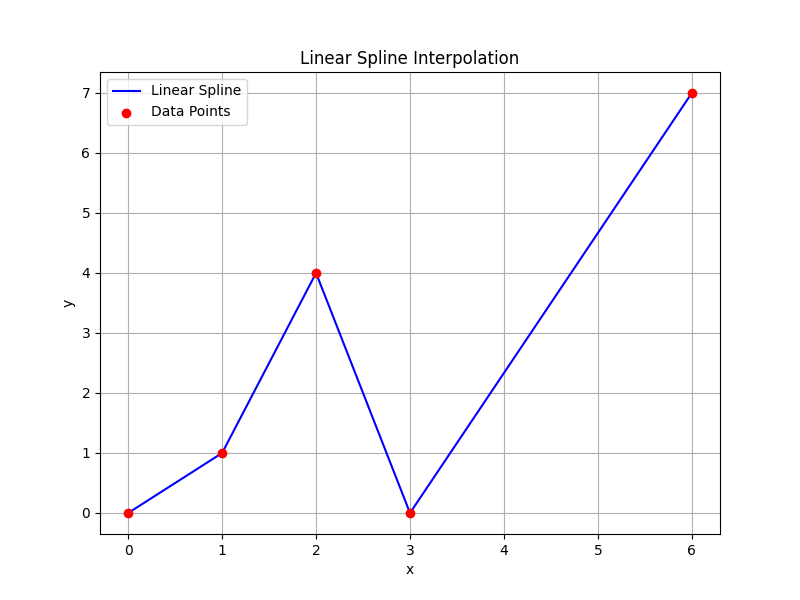
\includegraphics[width=\textwidth]{spline_plot_pp1.png}
      \caption{pp1的拟合结果}
  \end{minipage}\hfill
  \begin{minipage}{0.45\textwidth}
      \centering
      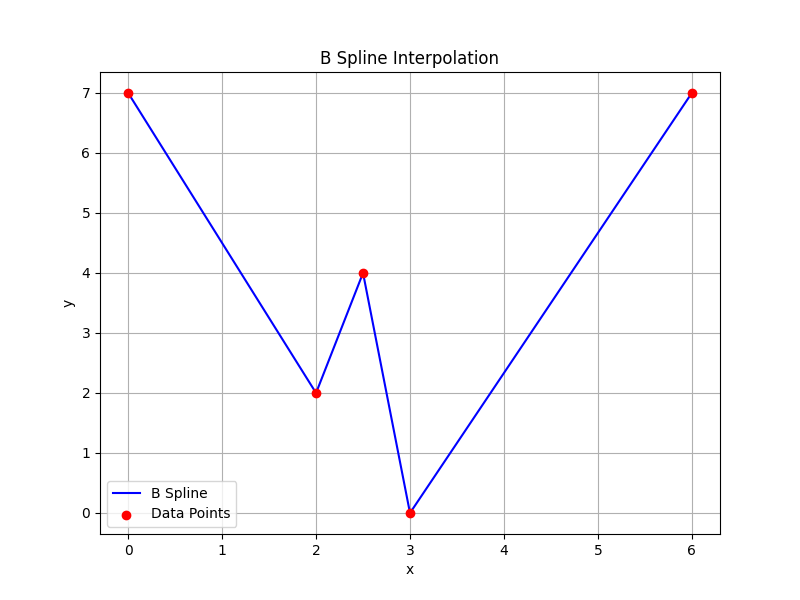
\includegraphics[width=\textwidth]{spline_plot_B1.png}
      \caption{1阶B-spline的拟合结果}
  \end{minipage}
\end{figure}
\subsection*{3阶样条的比对}
这里只展示在$natural$边界条件下二者的拟合效果.
\begin{figure}[h!]
  \centering
  \begin{minipage}{0.45\textwidth}
      \centering
      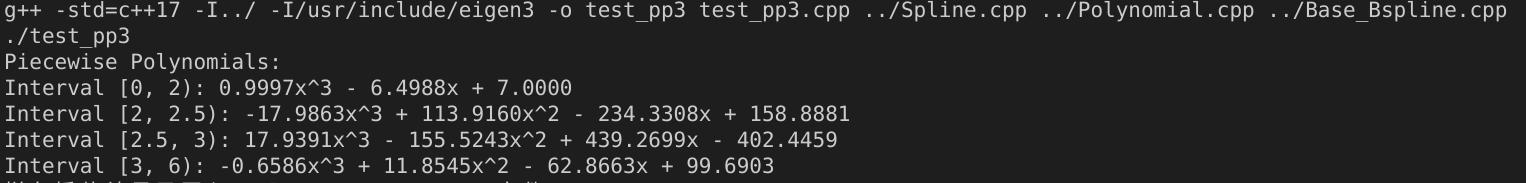
\includegraphics[width=\textwidth]{pp3.png}
      \caption{pp3的拟合结果}
  \end{minipage}\hfill
  \begin{minipage}{0.45\textwidth}
      \centering
      
\includegraphics[width=\textwidth]{B.png}
      \caption{3阶B-spline的拟合结果}
  \end{minipage}
\end{figure}

\begin{figure}[h!]
  \centering
  \begin{minipage}{0.45\textwidth}
      \centering
      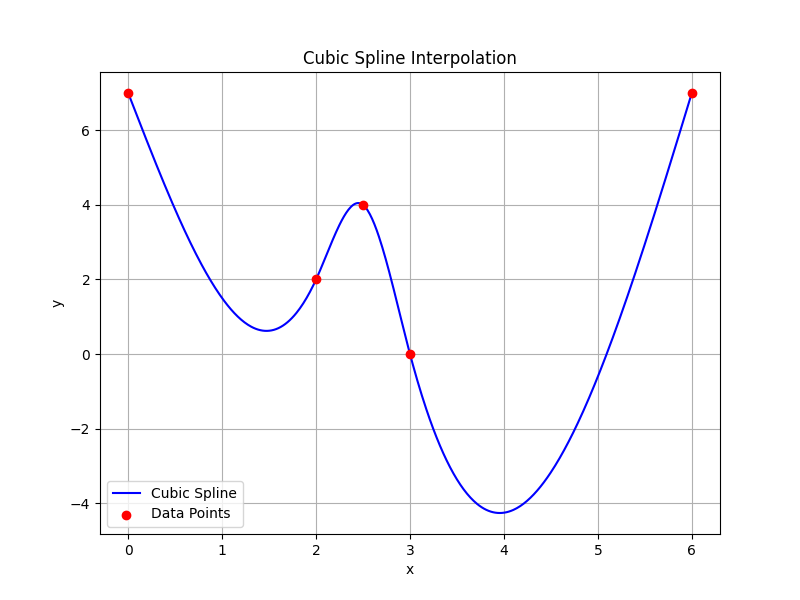
\includegraphics[width=\textwidth]{spline_plot_pp3.png}
      \caption{pp3的拟合结果}
  \end{minipage}\hfill
  \begin{minipage}{0.45\textwidth}
      \centering
      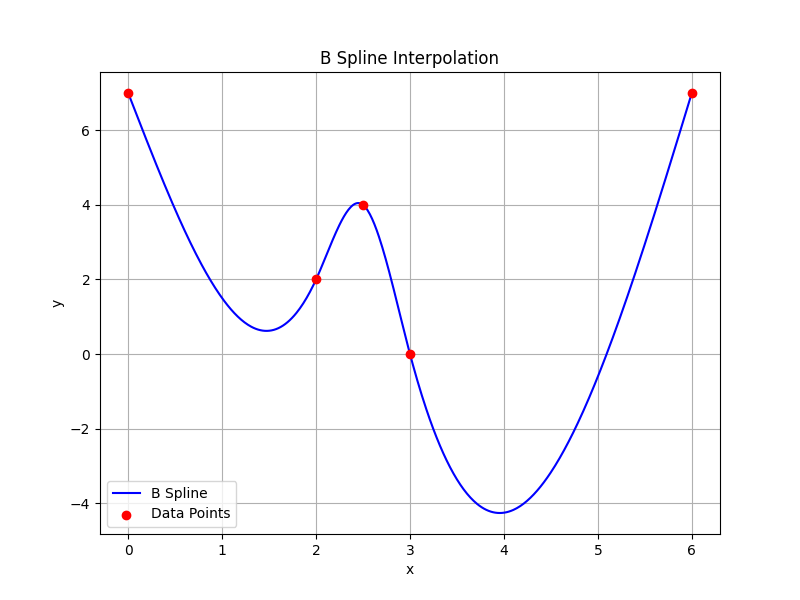
\includegraphics[width=\textwidth]{spline_plot_B.png}
      \caption{3阶B-spline的拟合结果}
  \end{minipage}
\end{figure}

\section*{\textbf{具体题目和分析}}
\subsection*{A}
\begin{figure}[H]
  \centering
  \begin{minipage}{0.45\textwidth}
      \centering
      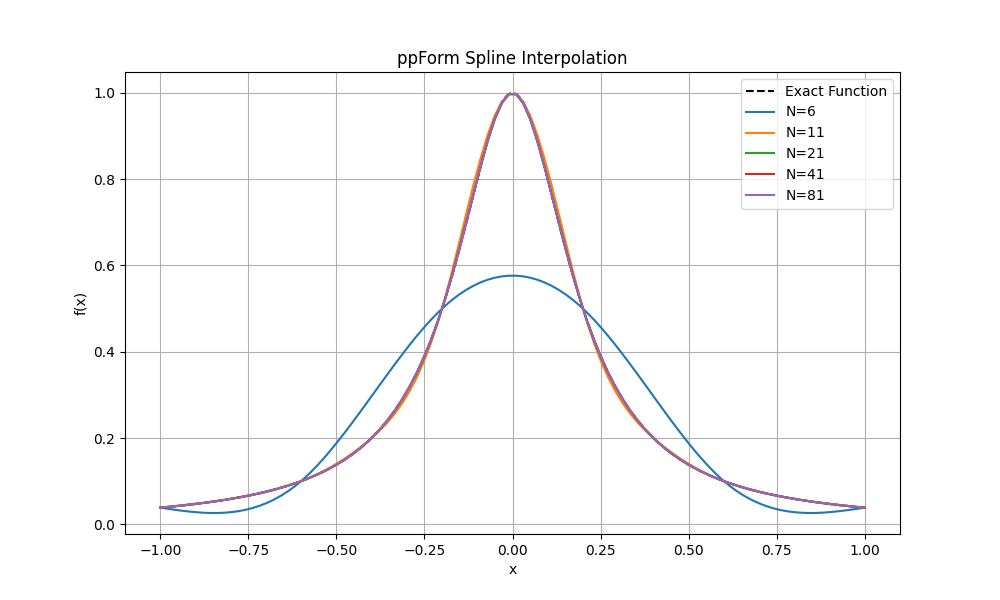
\includegraphics[width=\textwidth]{../pics/A_ppForm Spline Interpolation.png}
      \caption{pp3的拟合结果}
  \end{minipage}\hfill
  \begin{minipage}{0.45\textwidth}
      \centering
      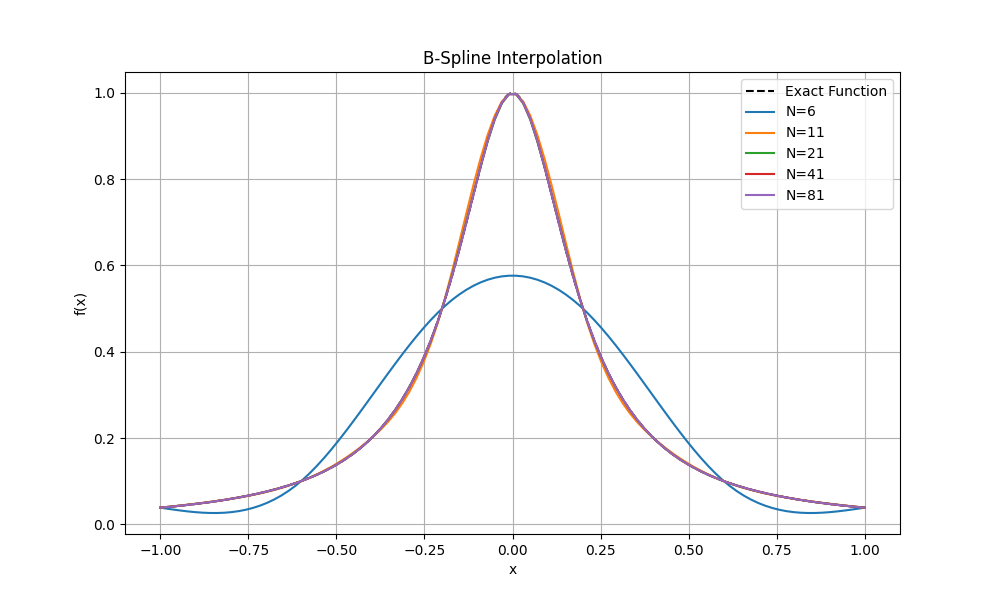
\includegraphics[width=\textwidth]{../pics/A_B-Spline Interpolation.png}
      \caption{3阶B-spline的拟合结果}
  \end{minipage}
\end{figure}

\subsection*{C}
\begin{figure}[H]
  \centering
  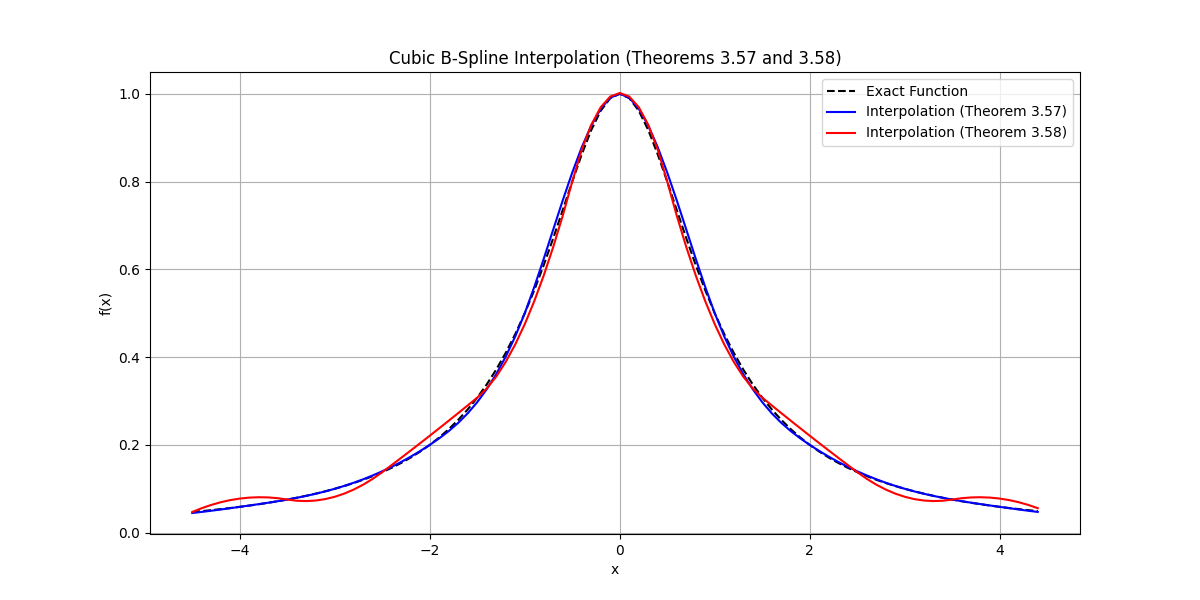
\includegraphics[width=0.8\textwidth]{../pics/C_interpolation_plot.png}
  \caption{B拟合效果}
\end{figure}

\subsection*{D}
\begin{figure}[h!]
  \centering
  \begin{minipage}{0.45\textwidth}
      \centering
      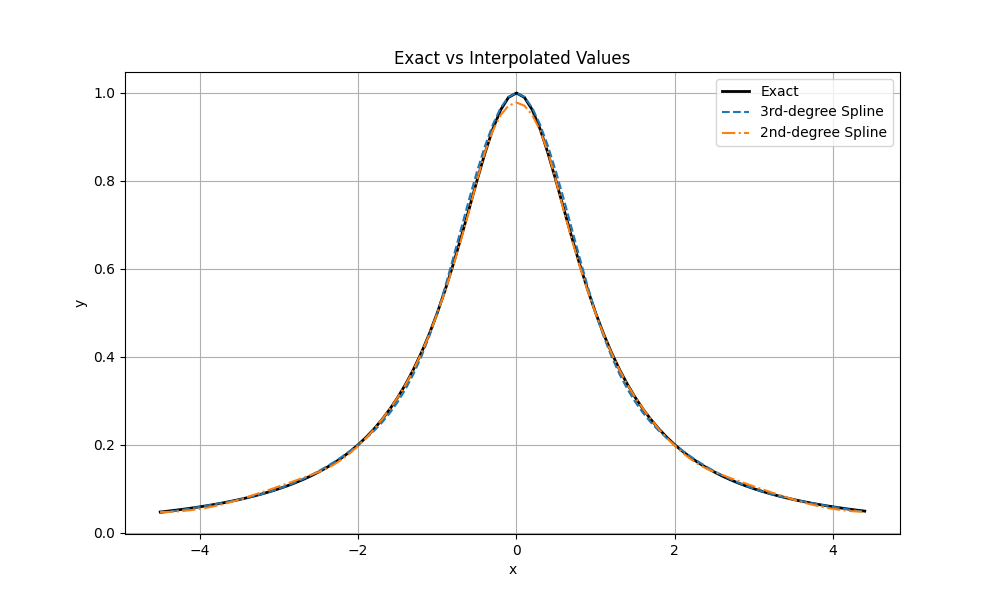
\includegraphics[width=\textwidth]{../pics/D_interpolation_plot.png}
      \caption{拟合结果}
  \end{minipage}\hfill
  \begin{minipage}{0.45\textwidth}
      \centering
      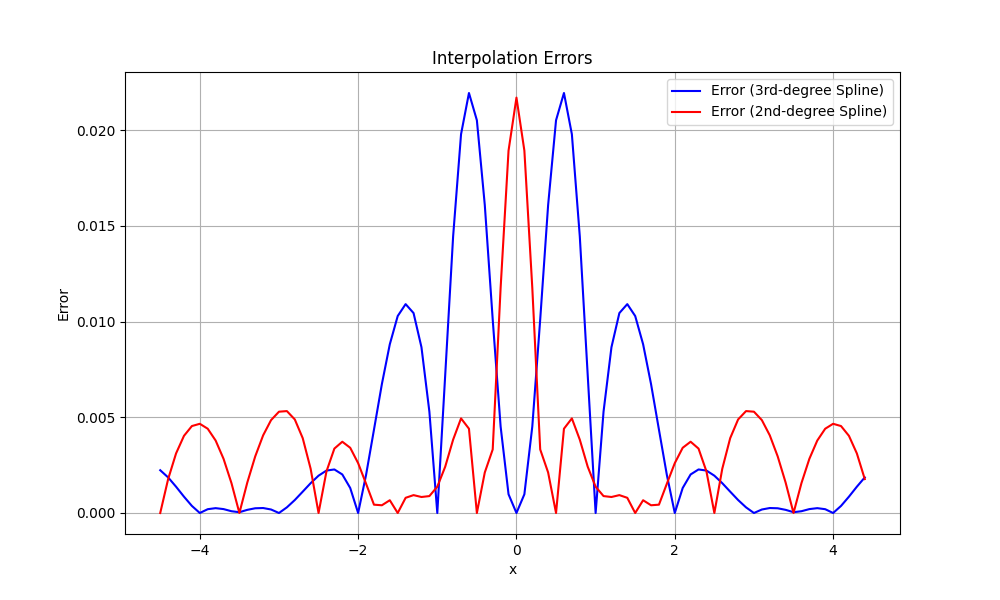
\includegraphics[width=\textwidth]{../pics/D_error_plot.png}
      \caption{误差}
  \end{minipage}
\end{figure}
\begin{center}
  \begin{tabular}{ccc}
      \toprule[1.5pt]
      \makebox[0.2\textwidth][c]{$x$} & \makebox[0.35\textwidth][c]{$E_s(x)$ of $S_2^1$} 
      & \makebox[0.35\textwidth][c]{$E_s(x)$ of $S_3^2$} \\
      \midrule[0.75pt]
      -3.5 & 6.93889e-017 & 0.000669568  \\
      -3   & 0.00141838   & 1.38778e-017 \\
      -0.5 & 1.11022e-016 & 0.0205289    \\
      0    & 0.120238     & 1.11022e-016 \\
      0.5  & 1.11022e-016 & 0.0205289    \\
      3    & 0.00141838   & 4.16334e-017 \\
      3.5  & 2.77556e-017 & 0.000669568  \\
      \bottomrule[1.5pt]
  \end{tabular}
\end{center}
除了机器误差，更进一步，考虑非插值节点处的最大误差并结合图像，可以发现 $S_3^2$ 的拟合精度要比 $S_2^1$ 
更高。这里一方面是由于三次函数具有更高的光滑形态，拟合上可以适应更高阶导数；另一方面是
由于待拟合函数为偶函数， $S_3^2$ 在拟合时选取了 0 点，该点对于原函数也是一个形态比较突出
的点，在该处放置插值节点的拟合精度会比不放置插值节点的拟合程度更好。

\subsection*{E}
下面的三组结果是选择了natural作为了边界条件.
\begin{figure}[h!]
  \centering
  \begin{minipage}{0.45\textwidth}
      \centering
      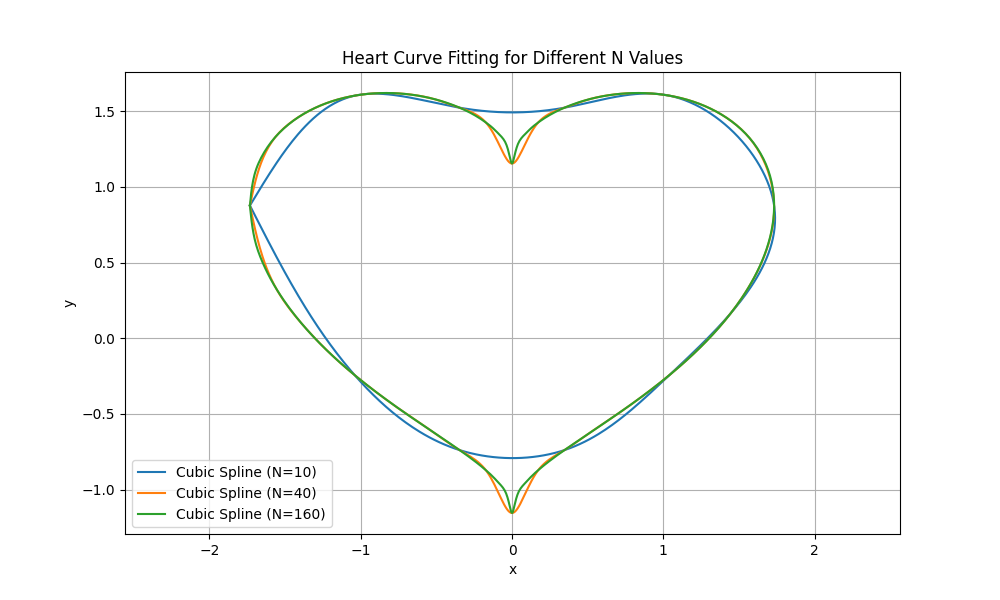
\includegraphics[width=\textwidth]{../pics/E1_heart_curve_comparison.png}
      \caption{cumulative chordal length拟合结果}
  \end{minipage}\hfill
  \begin{minipage}{0.45\textwidth}
      \centering
      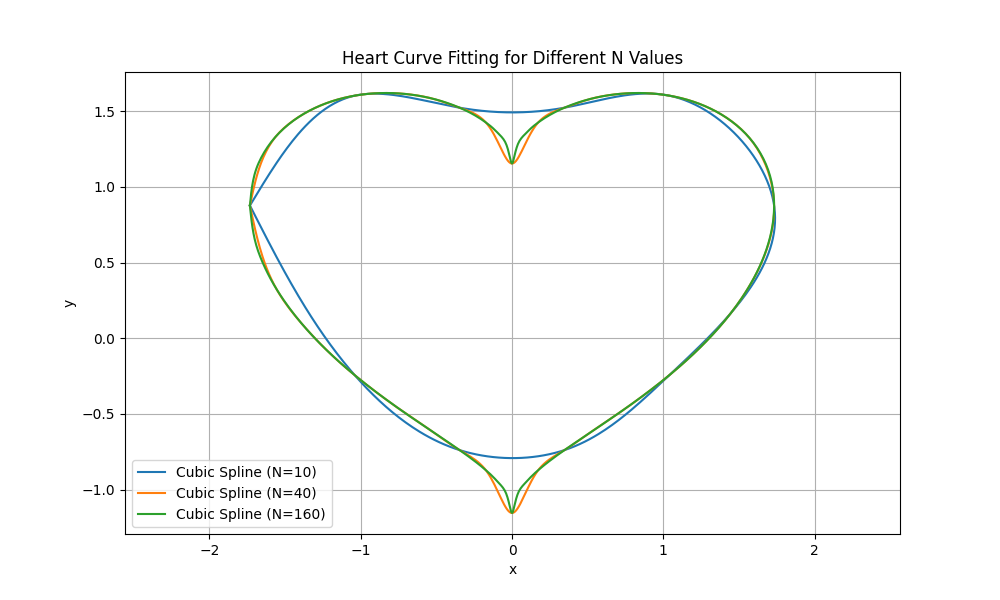
\includegraphics[width=\textwidth]{../pics/E1_heart_curve_comparison_2.png}
      \caption{等距离参数化拟合结果}
  \end{minipage}
\end{figure}

\begin{figure}[h!]
  \centering
  \begin{minipage}{0.45\textwidth}
      \centering
      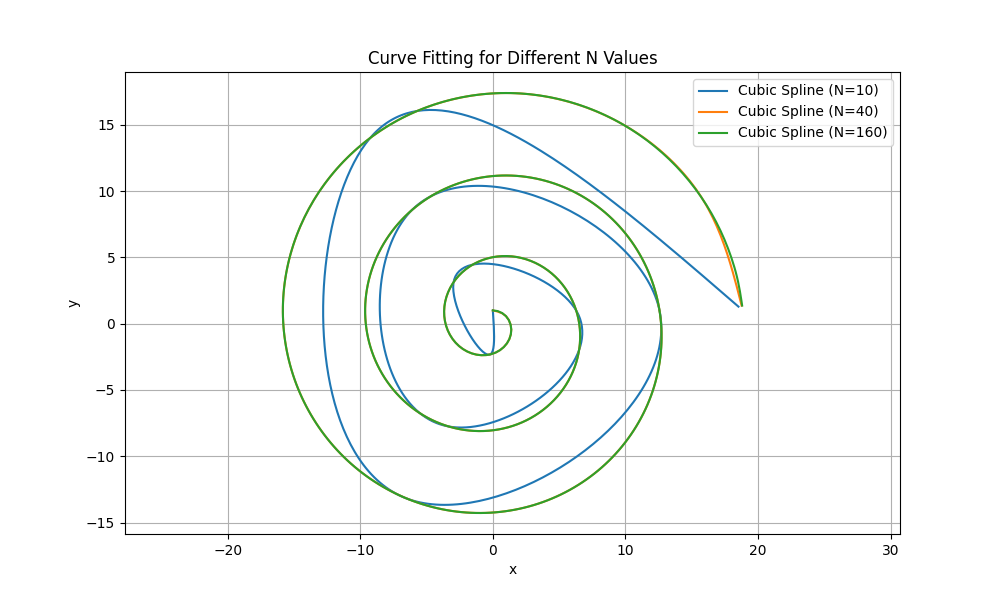
\includegraphics[width=\textwidth]{../pics/E2r2_curve_comparison.png}
      \caption{cumulative chordal length拟合结果}
  \end{minipage}\hfill
  \begin{minipage}{0.45\textwidth}
      \centering
      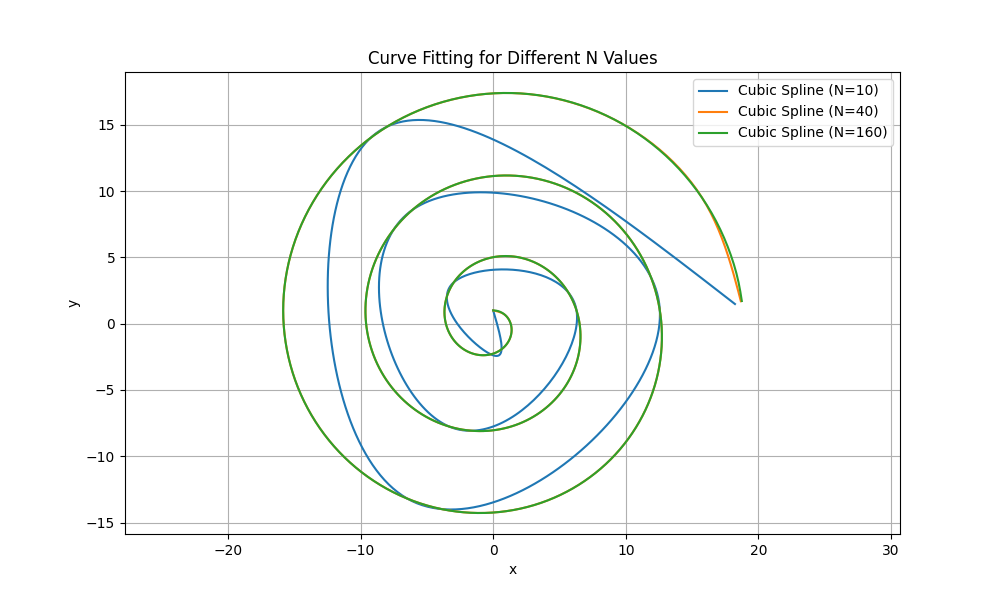
\includegraphics[width=\textwidth]{../pics/E2r2_curve_comparison_2.png}
      \caption{等距离参数化拟合结果}
  \end{minipage}
\end{figure}

\begin{figure}[h!]
  \centering
  \begin{minipage}{0.45\textwidth}
      \centering
      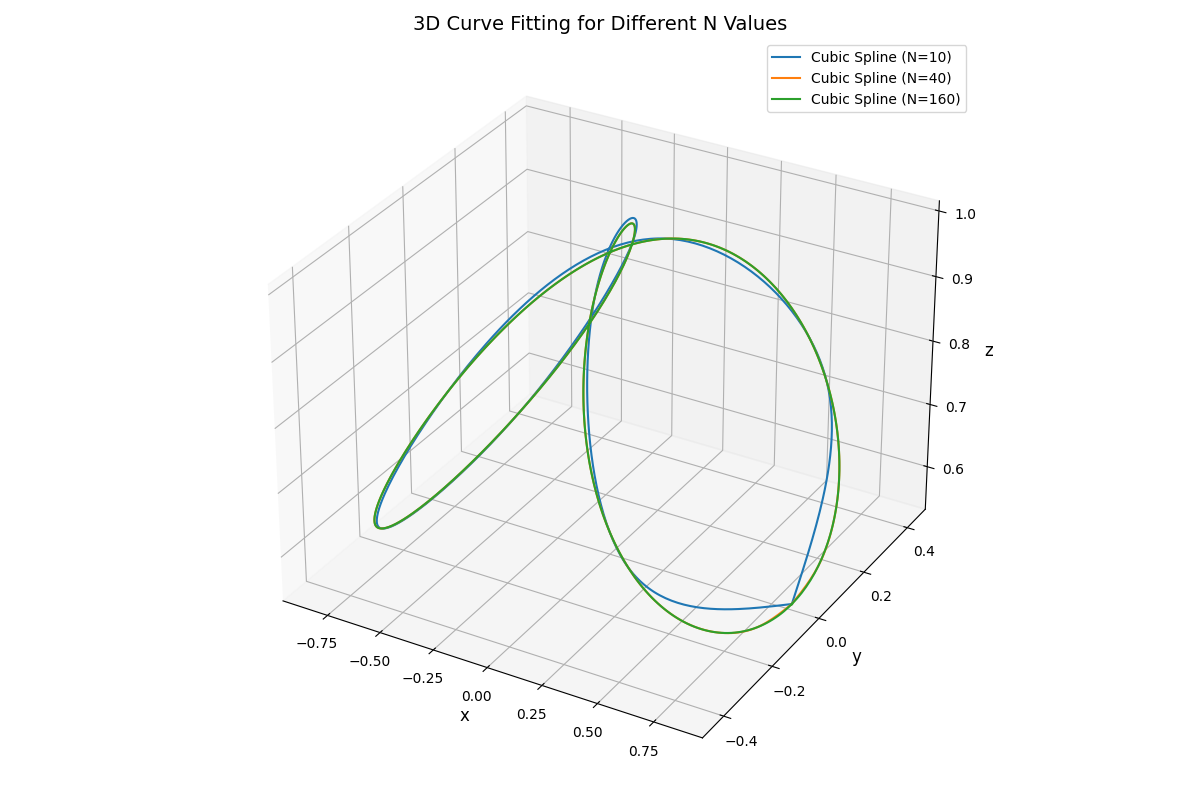
\includegraphics[width=\textwidth]{../pics/E3r3_curve_comparison_3d.png}
      \caption{cumulative chordal length拟合结果}
  \end{minipage}\hfill
  \begin{minipage}{0.45\textwidth}
      \centering
      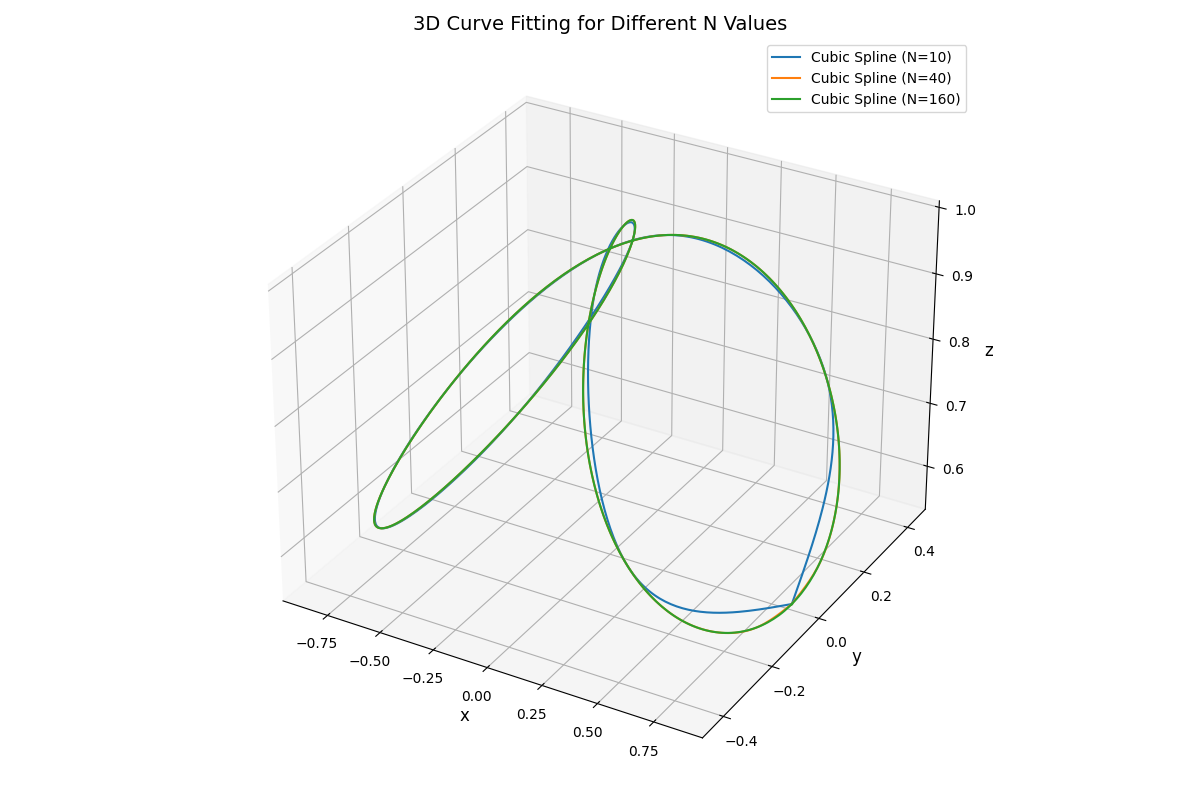
\includegraphics[width=\textwidth]{../pics/E3r3_curve_comparison_3d_2.png}
      \caption{等距离参数化拟合结果}
  \end{minipage}
\end{figure}
下面是选择了等弦长下的complete和periodic作为边界条件.
\begin{figure}[h!]
  \centering
  \begin{minipage}{0.45\textwidth}
      \centering
      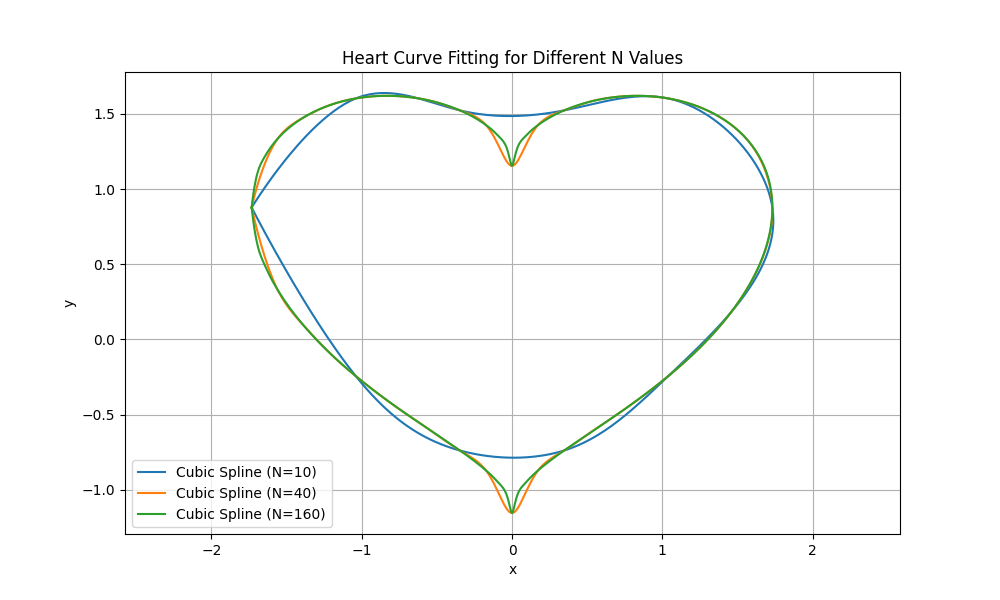
\includegraphics[width=\textwidth]{../pics/E1_complete.png}
      \caption{complete拟合结果}
  \end{minipage}\hfill
  \begin{minipage}{0.45\textwidth}
      \centering
      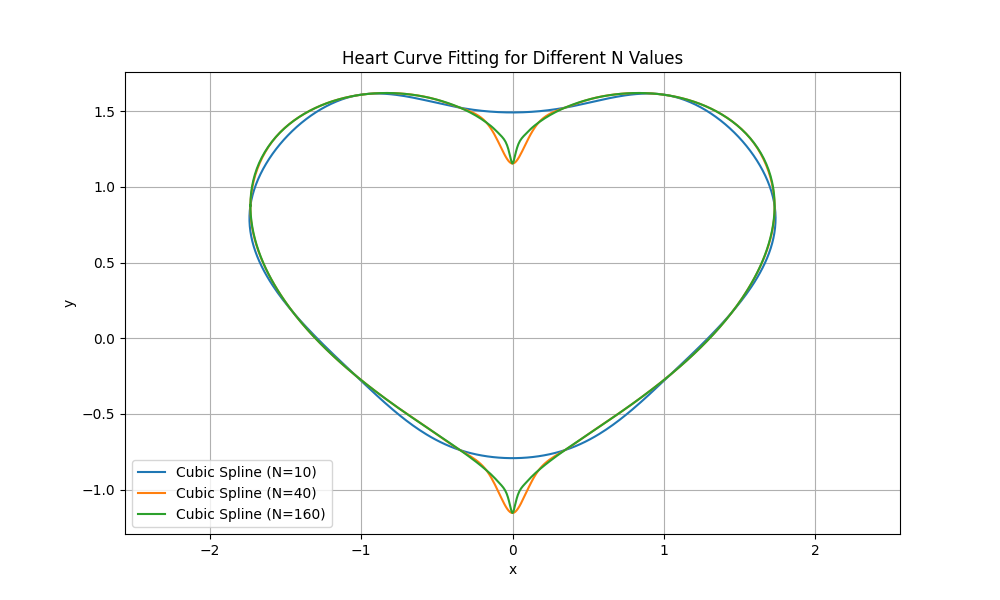
\includegraphics[width=\textwidth]{../pics/E1_periodic.png}
      \caption{periodic拟合结果}
  \end{minipage}
\end{figure}
\begin{figure}[h!]
  \centering
  \begin{minipage}{0.45\textwidth}
      \centering
      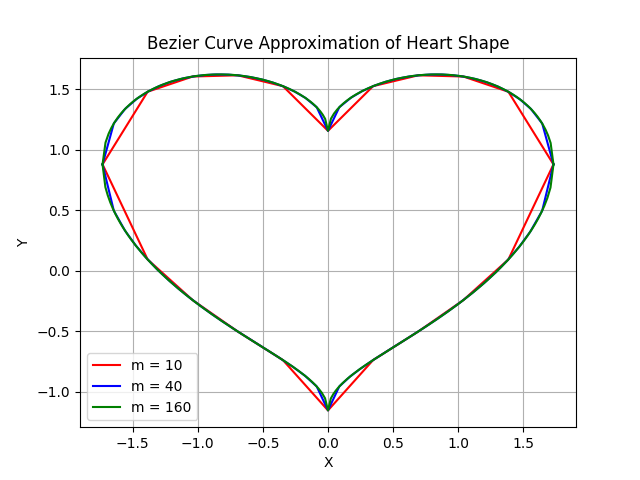
\includegraphics[width=\textwidth]{Bezier.png}
      \caption{Bezier拟合结果}
  \end{minipage}\hfill
  \begin{minipage}{0.45\textwidth}
      \centering
      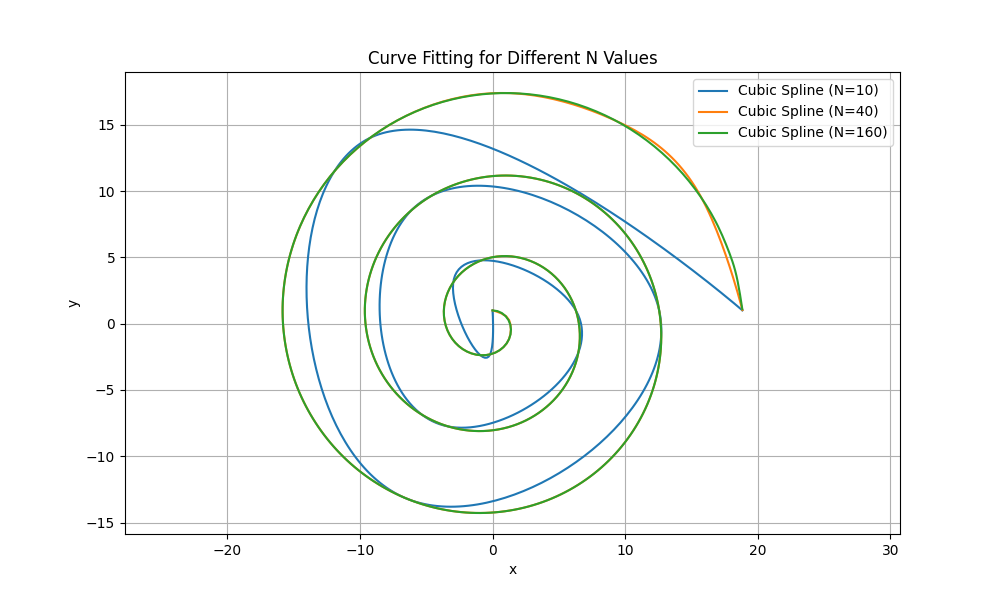
\includegraphics[width=\textwidth]{../pics/E2_complete.png}
      \caption{complete拟合结果}
  \end{minipage}
\end{figure}
\begin{figure}[H]
  \centering
  \begin{minipage}{0.45\textwidth}
      \centering
      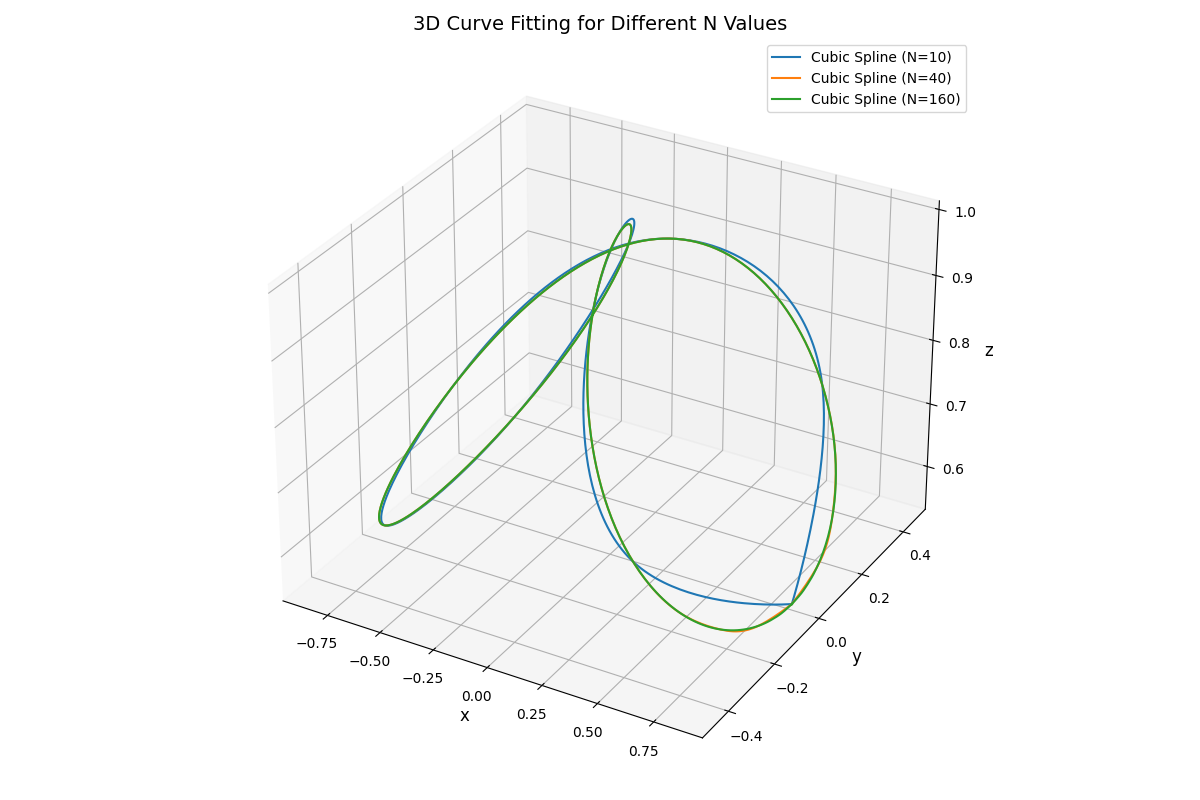
\includegraphics[width=\textwidth]{../pics/E3_complete.png}
      \caption{complete拟合结果}
  \end{minipage}\hfill
  \begin{minipage}{0.45\textwidth}
      \centering
      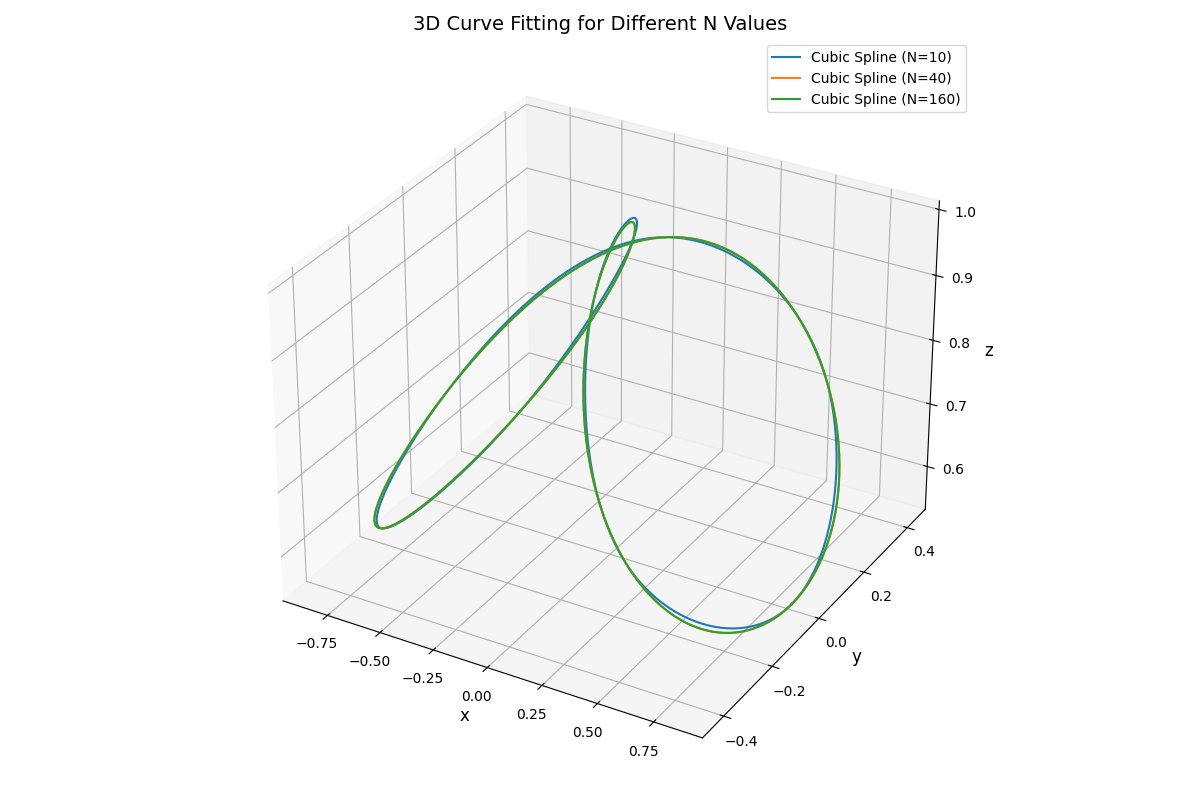
\includegraphics[width=\textwidth]{../pics/E3_periodic.png}
      \caption{periodic拟合结果}
  \end{minipage}
\end{figure}
\subsection*{F}
这道题目要求使用截断多项式的差分来计算出B样条基函数的结果. \cite*{openai2024chatgpt}
下面是3个结点的所做成的结果,即生成1阶基函数.
\begin{figure}[H]
  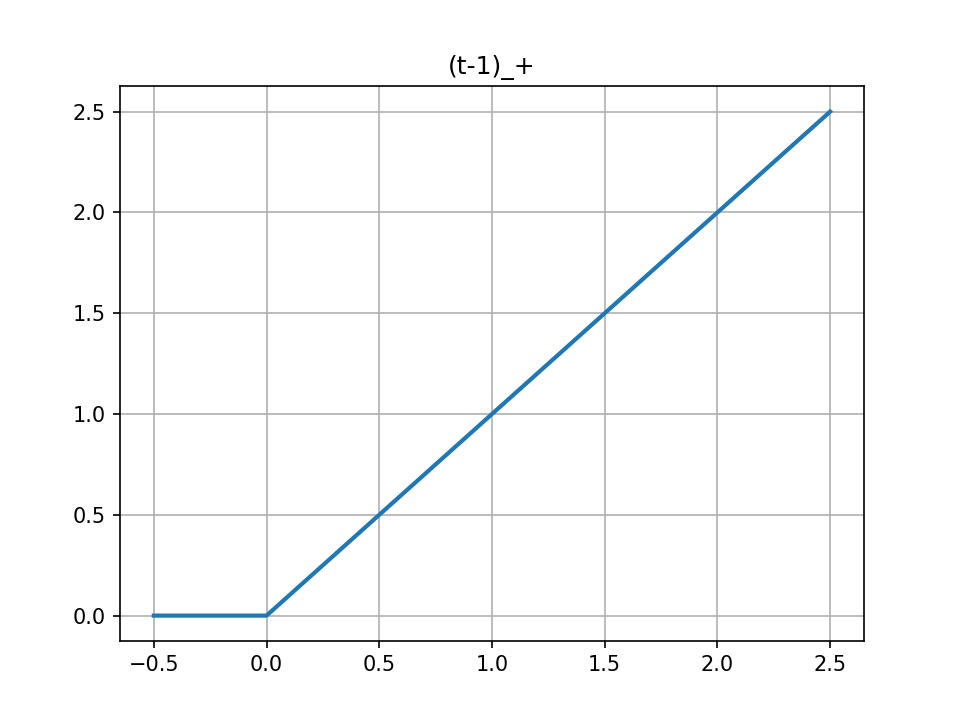
\includegraphics[width=0.3\textwidth]{../pics/fig1_0.png}
\end{figure}
\vspace{-40pt} % 调整两张图片之间的间距
\begin{figure}[H]
  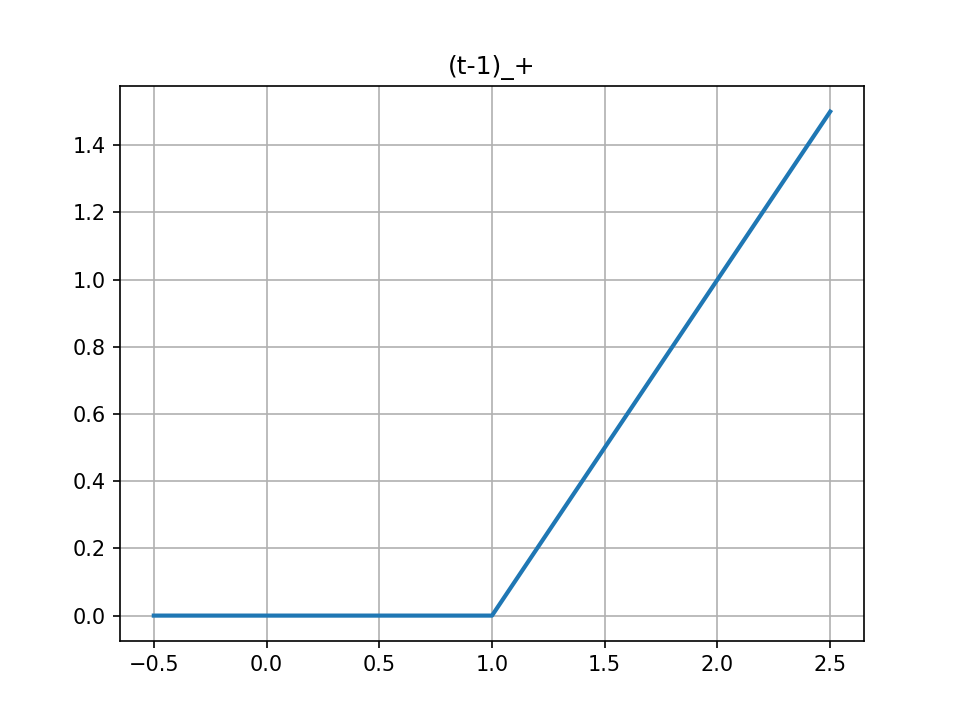
\includegraphics[width=0.3\textwidth]{../pics/fig1_1.png}
  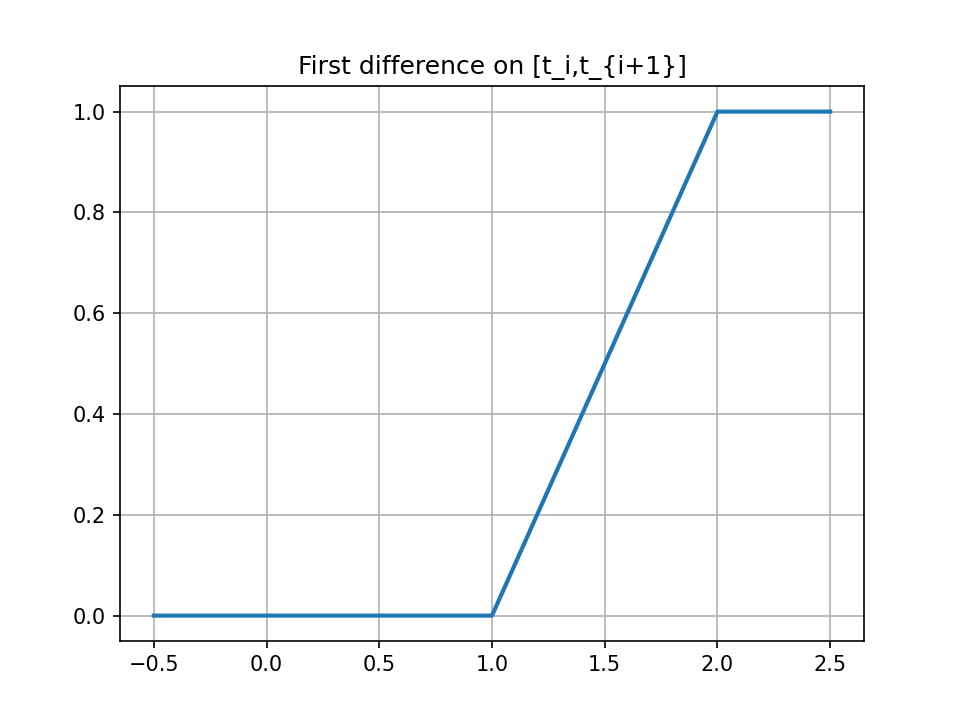
\includegraphics[width=0.3\textwidth]{../pics/fig2_1.png}
\end{figure}
\vspace{-40pt} % 调整两张图片之间的间距
\begin{figure}[H]
  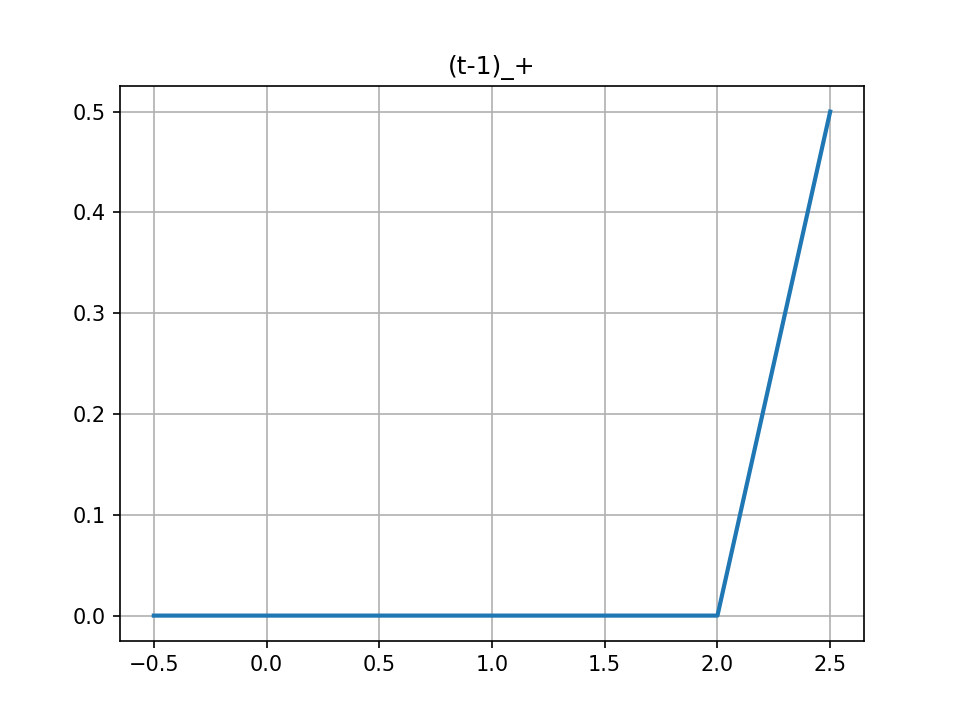
\includegraphics[width=0.3\textwidth]{../pics/fig1_2.png}
  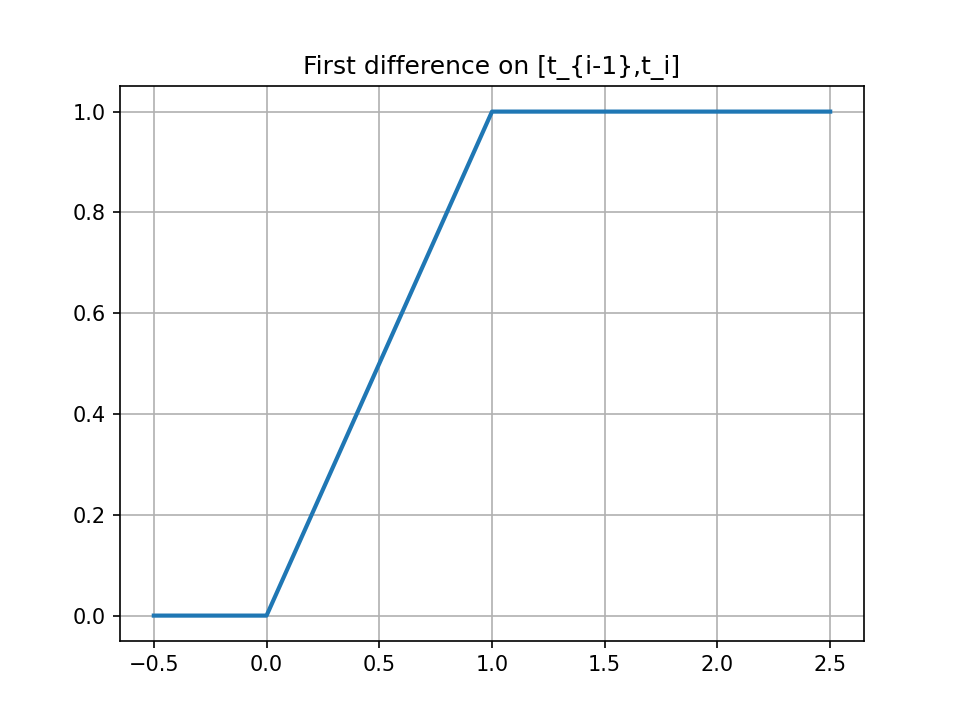
\includegraphics[width=0.3\textwidth]{../pics/fig2_2.png}
  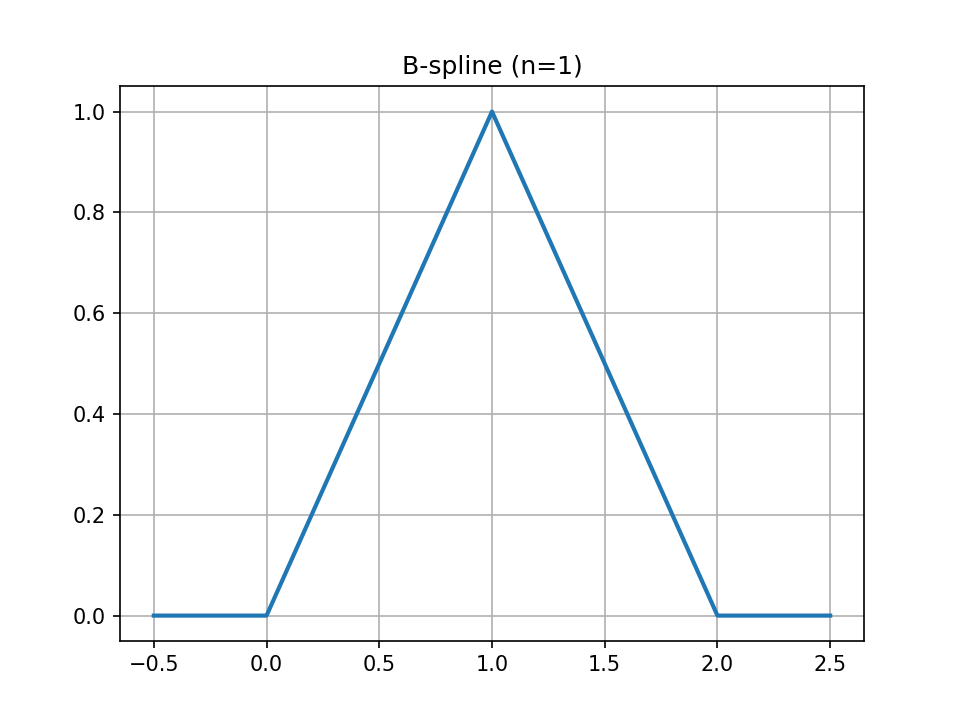
\includegraphics[width=0.3\textwidth]{../pics/fig3.png}
\end{figure}

下面是4个结点的所做成的结果,即生成2阶基函数.
\begin{figure}[H]
  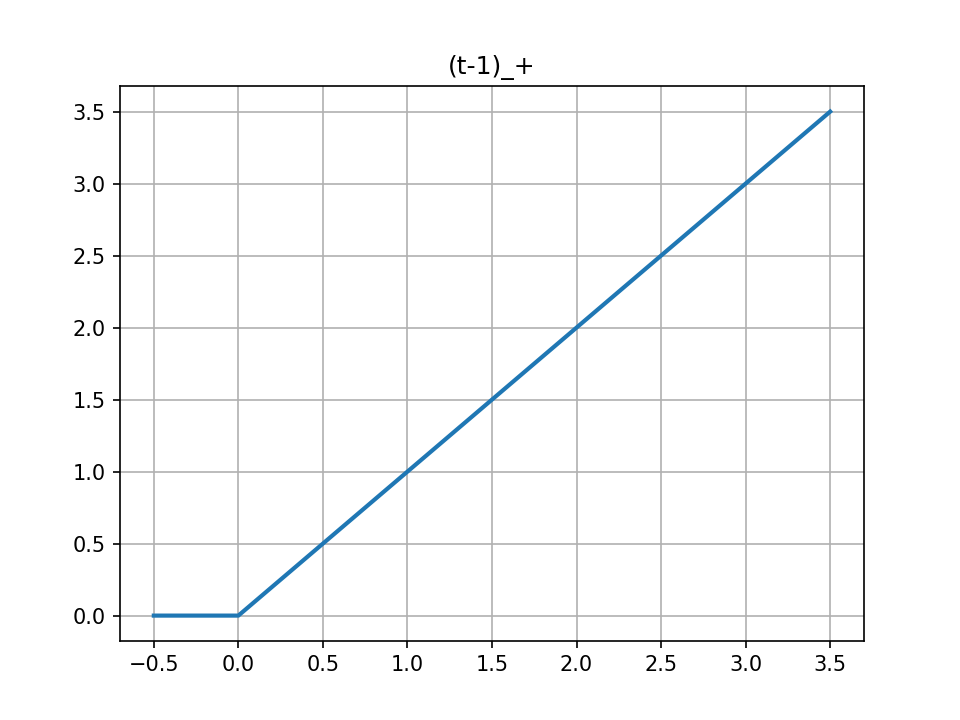
\includegraphics[width=0.2\textwidth]{../pics/2_fig1_0.png}
\end{figure}
\vspace{-40pt} % 调整两张图片之间的间距
\begin{figure}[H]
  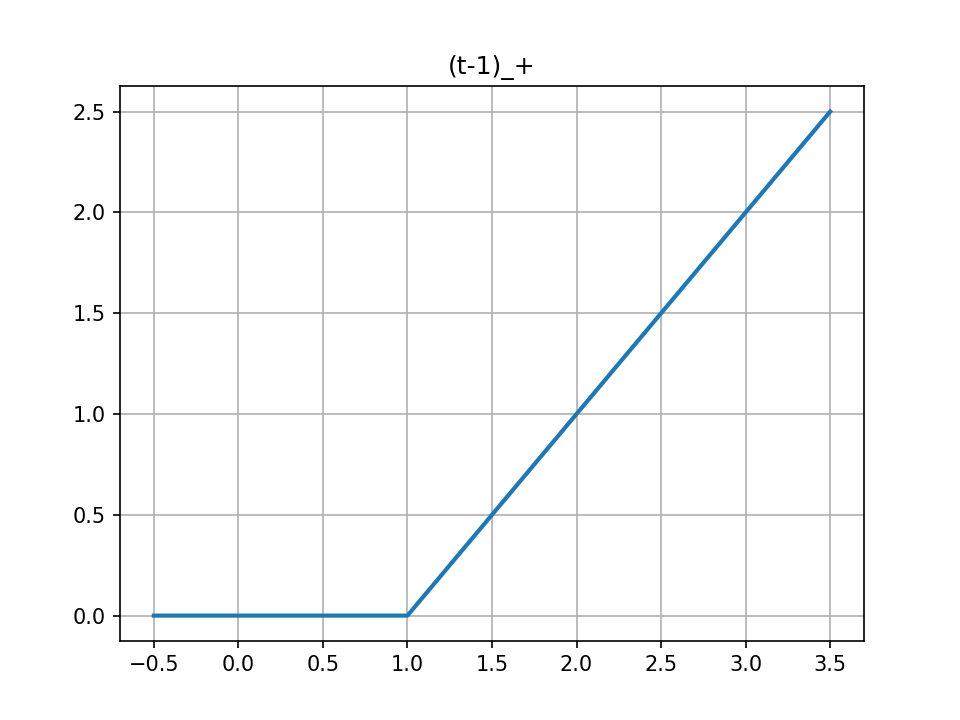
\includegraphics[width=0.2\textwidth]{../pics/2_fig1_1.png}
  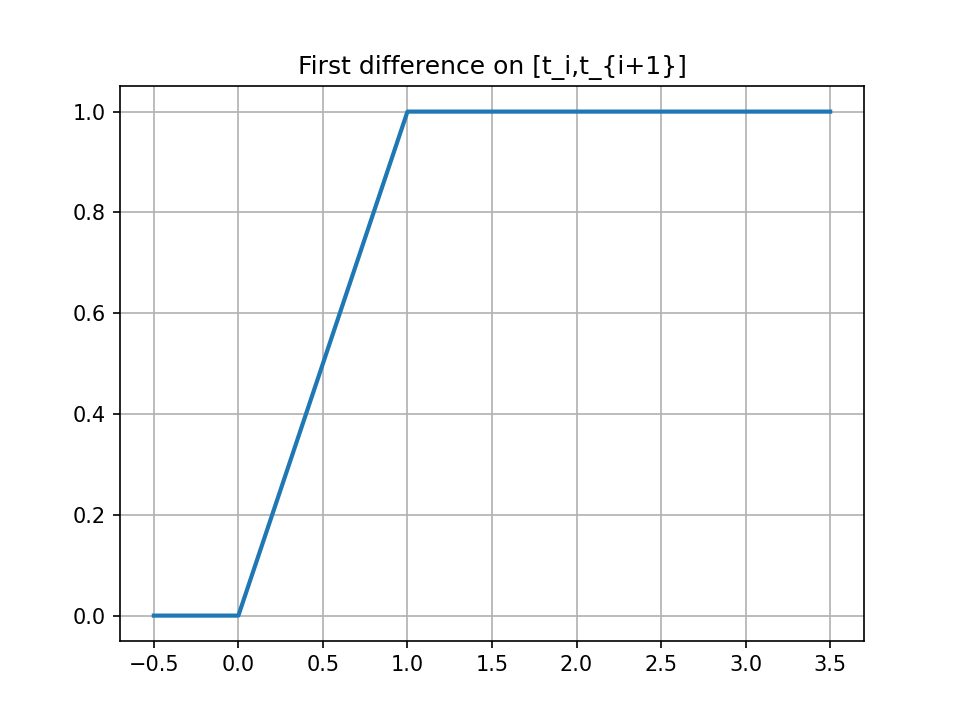
\includegraphics[width=0.2\textwidth]{../pics/2_fig2_1.png}
\end{figure}

\begin{figure}[H]
  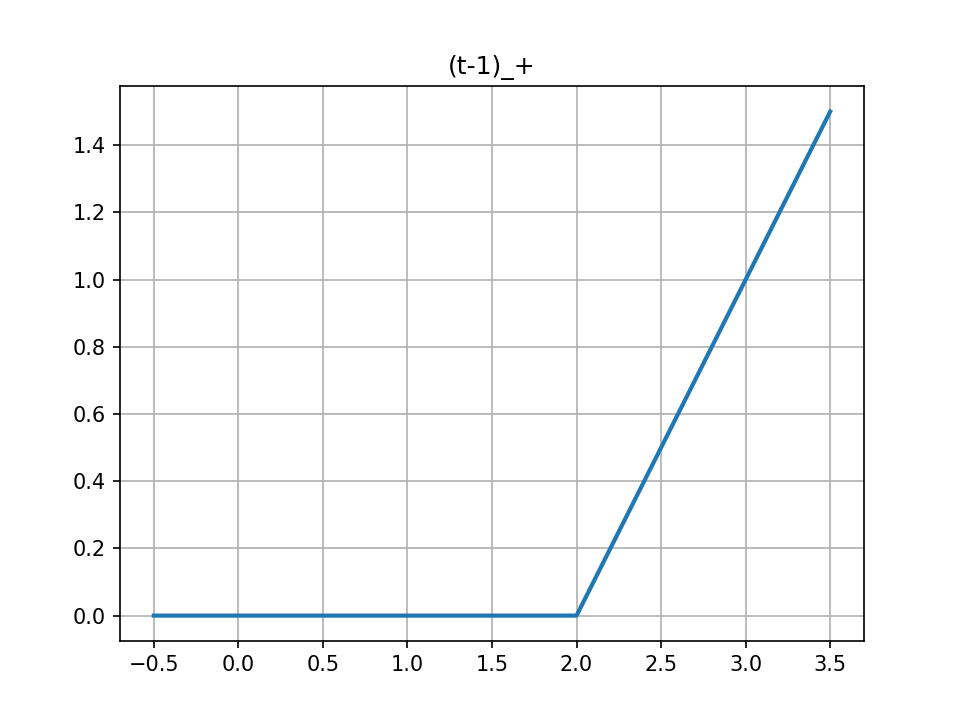
\includegraphics[width=0.2\textwidth]{../pics/2_fig1_2.png}
  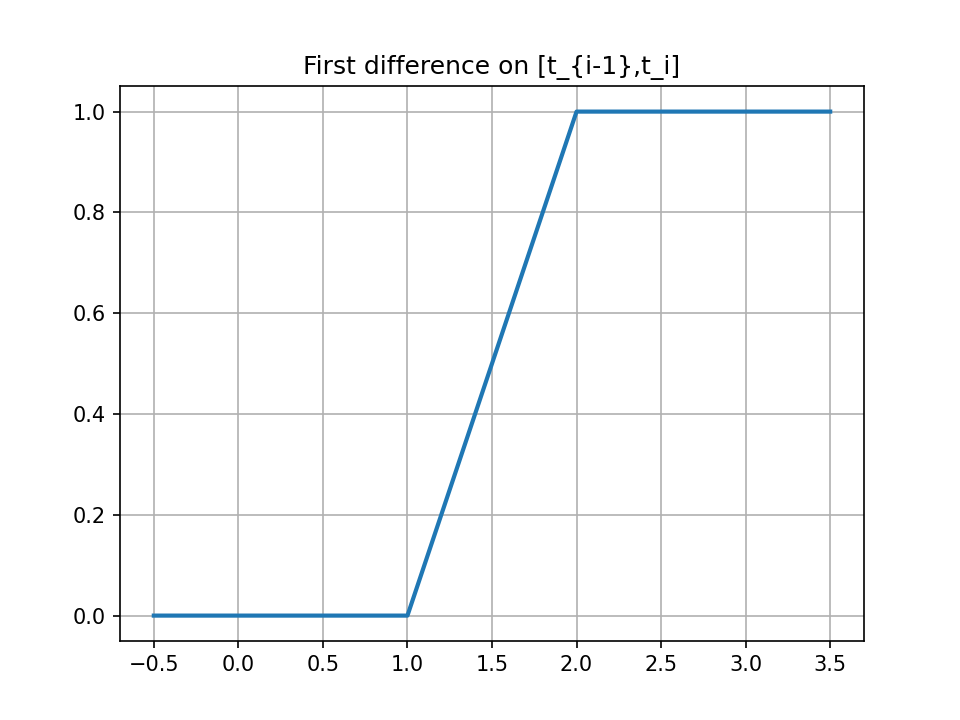
\includegraphics[width=0.2\textwidth]{../pics/2_fig2_2.png}
  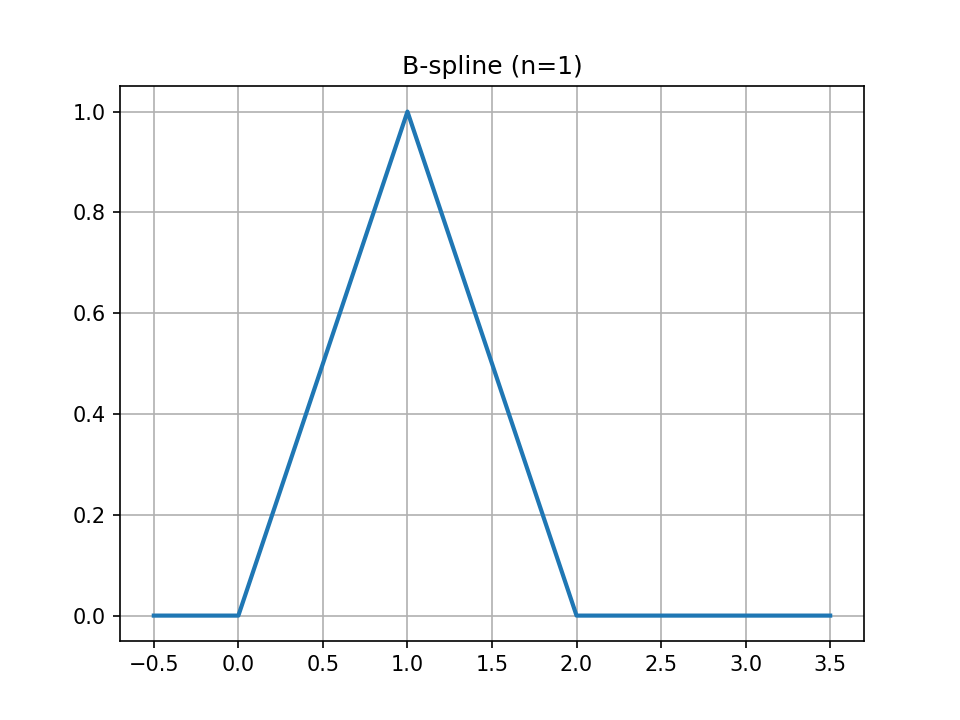
\includegraphics[width=0.2\textwidth]{../pics/2_fig3_1.png}
\end{figure}

\begin{figure}[H]
  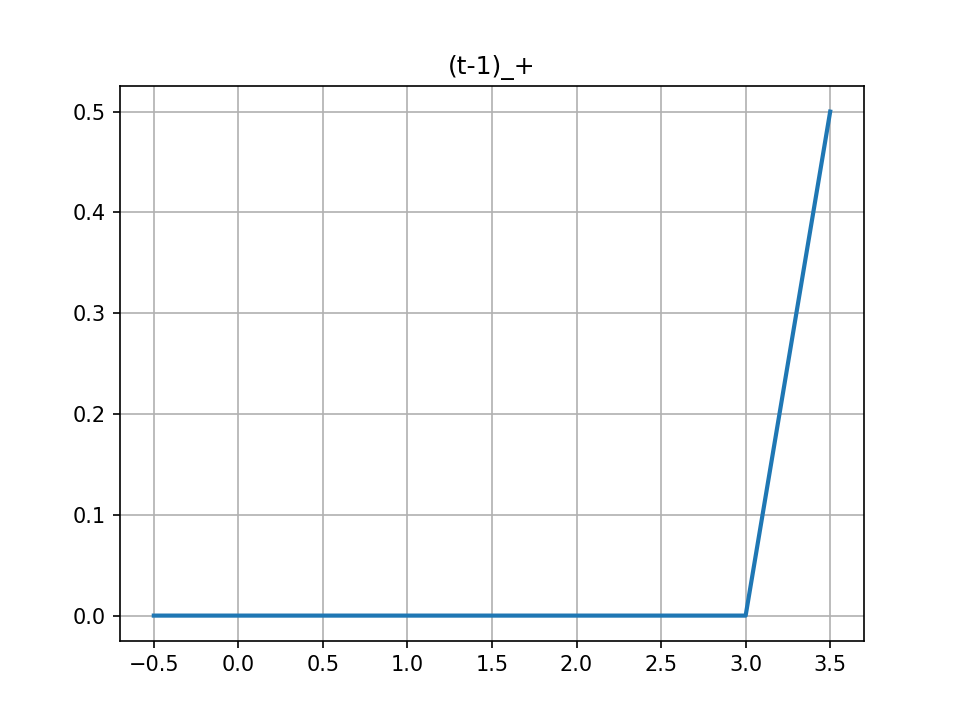
\includegraphics[width=0.2\textwidth]{../pics/2_fig1_3.png}
  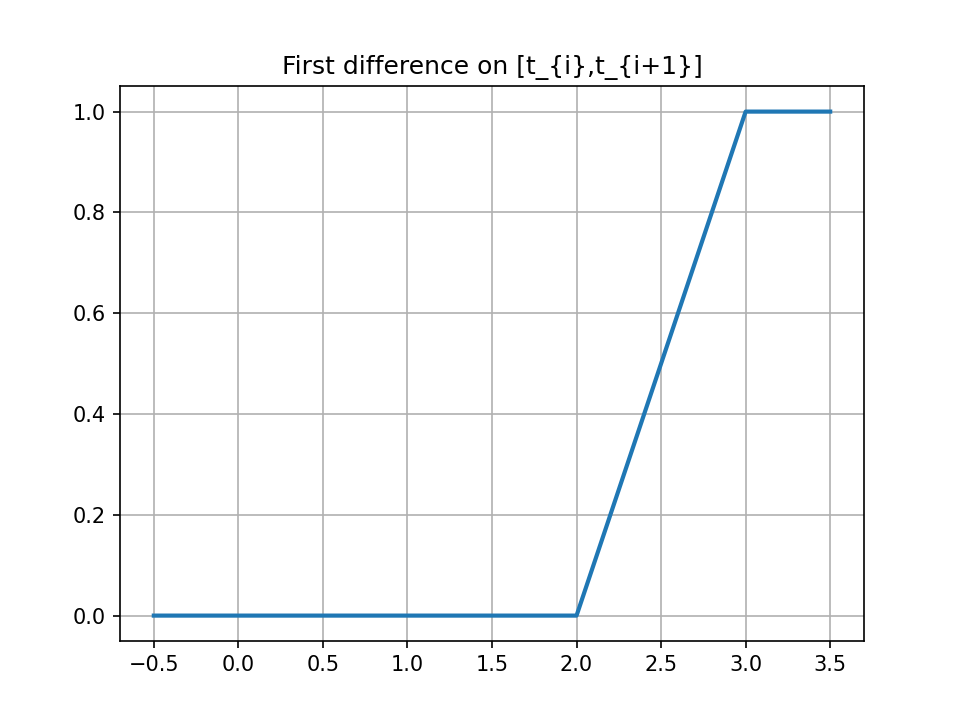
\includegraphics[width=0.2\textwidth]{../pics/2_fig2_3.png}
  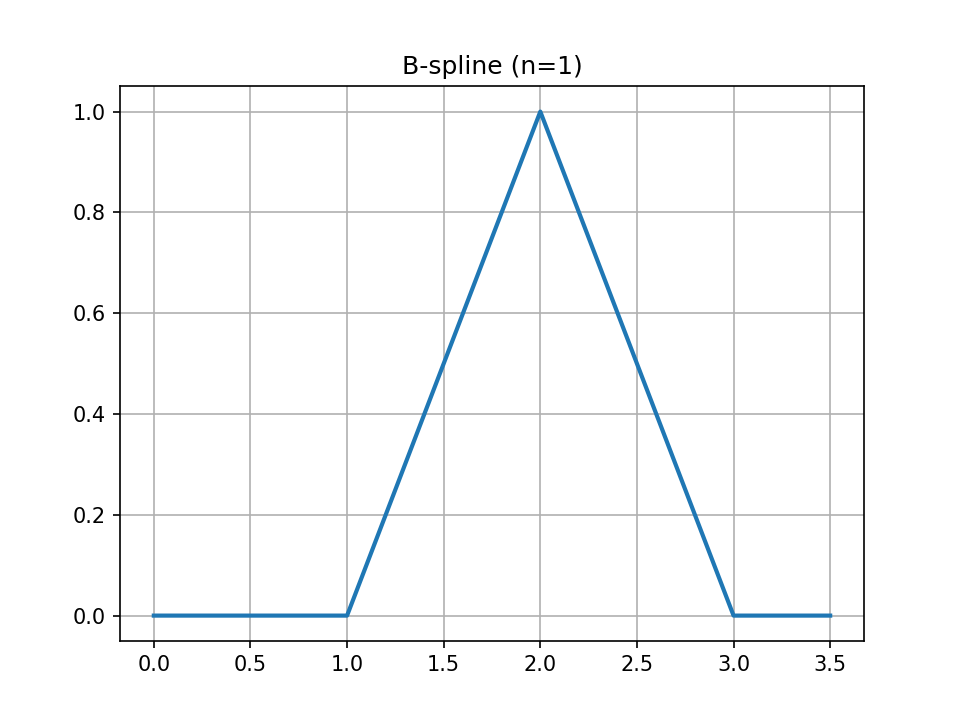
\includegraphics[width=0.2\textwidth]{../pics/2_fig3_2.png}
  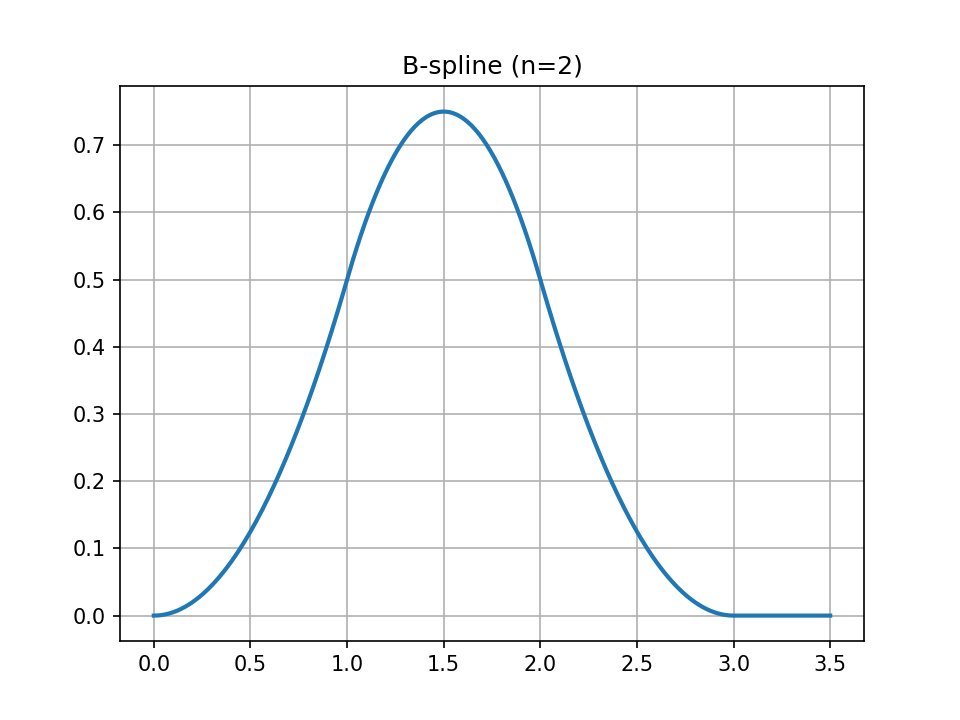
\includegraphics[width=0.2\textwidth]{../pics/2_fig4.png}
\end{figure}
% ==============================================
\section*{ \center{\normalsize {Acknowledgement}} }
\printbibliography

\end{document}